%% abtex2-modelo-trabalho-academico.tex, v-1.9.2 laurocesar
%% Copyright 2012-2014 by abnTeX2 group at http://abntex2.googlecode.com/ 
%%
%% This work may be distributed and/or modified under the
%% conditions of the LaTeX Project Public License, either version 1.3
%% of this license or (at your option) any later version.
%% The latest version of this license is in
%%   http://www.latex-project.org/lppl.txt
%% and version 1.3 or later is part of all distributions of LaTeX
%% version 2005/12/01 or later.
%%
%% This work has the LPPL maintenance status `maintained'.
%% 
%% The Current Maintainer of this work is the abnTeX2 team, led
%% by Lauro C�sar Araujo. Further information are available on 
%% http://abntex2.googlecode.com/
%%
%% This work consists of the files abntex2-modelo-trabalho-academico.tex,
%% abntex2-modelo-include-comandos and abntex2-modelo-references.bib
%%

% ------------------------------------------------------------------------
% ------------------------------------------------------------------------
% abnTeX2: Modelo de Trabalho Academico (tese de doutorado, dissertacao de
% mestrado e trabalhos monograficos em geral) em conformidade com 
% ABNT NBR 14724:2011: Informacao e documentacao - Trabalhos academicos -
% Apresentacao
% ------------------------------------------------------------------------
% ------------------------------------------------------------------------

\documentclass[en]{ufpethesis}

\usepackage{graphicx}			% Inclus�o de gr�ficos
\usepackage{caption}
\usepackage{subcaption}
\usepackage[table,xcdraw]{xcolor}
\usepackage{tabularx,ragged2e}
\usepackage{algorithm}% http://ctan.org/pkg/algorithms
\usepackage{algpseudocode}% http://ctan.org/pkg/algorithmicx
\newcolumntype{Y}{>{\raggedright\arraybackslash}X} % right "X" column
\newcolumntype{Z}{>{\raggedleft\arraybackslash}X} % left "X" column
\usepackage{sectsty}
\usepackage{ textcomp }
\usepackage[utf8]{inputenc}
\usepackage{setspace}
\usepackage{listings}
\usepackage[T1]{fontenc}
\sectionfont{\bfseries\Large\raggedright}

\renewcommand{\baselinestretch}{1.5} %espa�amento de linhas
\setlength{\parindent}{1.5cm}

\let\Algorithm\algorithm
\renewcommand\algorithm[1][]{\Algorithm[#1]\setstretch{1}}

%% Identifica��o:

% Universidade
% e.g. \university{Universidade de Campinas}
% Na UFPE, comente a linha a seguir
\university{Universidade Federal de Pernambuco}

% Endere�o (cidade)
% e.g. \address{Campinas}
% Na UFPE, comente a linha a seguir
\address{Recife}

% Instituto ou Centro Acad�mico
% e.g. \institute{Centro de Ci�ncias Exatas e da Natureza}
% Comente se n�o se aplicar
\institute{Centro de Inform\'{a}tica}

% Departamento acad�mico
% e.g. \department{Departamento de Inform�tica}
% Comente se n�o se aplicar
\department{Departamento de Inform\'{a}tica}

% Programa de p�s-gradua��o
% e.g. \program{P�s-gradua��o em Ci�ncia da Computa��o}
\program{P\'{o}s-gradua\c{c}\~{a}o em Ci\^{e}ncia da Computa\c{c}\~{a}o}

% �rea de titula��o
% e.g. \majorfield{Ci�ncia da Computa��o}
\majorfield{Ci\^{e}ncia da Computa\c{c}\~{a}o}

% T�tulo da disserta��o/tese
% e.g. \title{Sobre a conjectura $P=NP$}
\title{Using OLAP Queries for Data Analysis on Graph Databases}

% Data da defesa
% e.g. \date{19 de fevereiro de 2003}
\date{21 de agosto de 2017}

% Autor
% e.g. \author{Jos� da Silva}
\author{Nicolle Chaves Cysneiros}

% Orientador(a)
% Op��o: [f] - para orientador do sexo feminino
% e.g. \adviser[f]{Profa. Dra. Maria Santos}
\adviser[f]{Prof\textordfeminine. Dr\textordfeminine. Ana Carolina Salgado}

% ----
% In�cio do documento
% ----
\begin{document}

\frontmatter
\frontpage
\presentationpage

\resumo
Bancos de Dados (BDs) em Grafo s\~{a}o uma alternativa aos tradicionais BDs Relacionais e permitem uma melhor escalabilidade do sistema, al\'{e}m de uma maneira mais natural de representar dados altamente conectados. Os BDs em Grafo tamb\'{e}m permitem diferentes tipos de an\'{a}lises em grafos, como medidas de centralidade e algoritmos de detec\c{c}\~{a}o de comunidades. Apesar disso, ainda n\~{a}o existem ferramentas dispon\'{i}veis no mercado para fazer an\'{a}lise multidimensional em grafos, como os sistemas OLAP existentes que operam sobre BDs Relacionais. No meio acad\^{e}mico, existem algumas propostas de frameworks que visam a constru\c{c}\~{a}o de um cubo multidimensional composto por grafos agregados, obtidos a partir da combina\c{c}\~{a}o de n\'{o}s e arestas do grafo original de acordo com as dimens\~{o}es e medidas analisadas. Contudo, a maior parte das pesquisas s\~{a}o voltadas para a an\'{a}lise de grafos homog\^{e}neos, enquanto os trabalhos que se dedicam a grafos heterog\^{e}neos realizam a an\'{a}lise multidimensional a partir de um modelo intermedi\'{a}rio do dado original. Esse projeto prop\~{o}e um sistema para a realiza\c{c}\~{a}o de consultas OLAP em um Banco de Dados em Grafo sem a necessidade da gera\c{c}\~{a}o de um modelo intermedi\'{a}rio de dados para realizar an\'{a}lise em grafos heterog\^{e}neos. O sistema proposto \'{e} capaz de responder consultas OLAP a partir de grafos agregados extra\'{i}dos do grafo original, al\'{e}m de tamb\'{e}m realizar an\'{a}lises acerca da topologia do grafo. Neste trabalho s\~{a}o apresentados experimentos mostrando a efic\'{a}cia do sistema para responder \`{a}s consultas anal\'{i}ticas e compara\c{c}\~{o}es espec\'{i}ficas entre o sistema descrito e as solu\c{c}\~{o}es existentes.
% Palavras-chave do resumo em Portugu�s
\begin{keywords}
OLAP, Bando de Dados em Grafo, Grafos, Data Analysis
\end{keywords}

\tableofcontents
\listoffigures
% ----------------------------------------------------------
% ELEMENTOS TEXTUAIS
% ----------------------------------------------------------
\mainmatter

% ----------------------------------------------------------
% Introduction
% ----------------------------------------------------------
\chapter{Introduction}
% ----------------------------------------------------------

% ---
% Fundamentals
% ---
\chapter{OLAP and Graph Databases}
% ---
This chapter introduces the main concepts that forms the theoretical foundation necessary to better understand the work presented in this dissertation. Initially, we will explore the definition of Data Warehouse, Multidimensional Model and OLAP tools. Then, we will dive into concepts related to Graph and Graph Databases.

\section{Data Warehouse}
According to \cite{Inmon2005}, a data warehouse (DW) is ``a subject-oriented, integrated, nonvolatile, and time-variant collection of data in support of management's decisions''. The first important aspect of a data warehouse is that it is subject-oriented, which means that the information stored in the DW is related to the company's subject. Consider a retail company for example: the main subjects can be product, sale, vendor and customer, therefore the data in the warehouse will be related to these entities.
 
The second characteristic of a data warehouse is that it is integrated, which means it contains data coming from multiple different sources. During the process of loading the warehouse, the data is converted, formatted, normalised and go through any other process to make the final information stored in the warehouse consistent. Another important aspect of a data warehouse is that it is nonvolatile, which means that the data in the warehouse does not get updated as operational environment. The warehouse is loaded in batches and it stores a snapshot, creating a history of the data. The final important aspect of a DW is that every record of data contains some sort of a time attribute to mark the moment in which the record is accurate.
 
Figure \ref{fig:figure1} shows the basic elements of a data warehouse \cite{Kimball2011}. The Operational Source Systems capture and store the transactions of the business and they are considered elements outside of the data warehouse, since there is no control on the content or the format of the data that they store. The Data Staging Area is where the process of Extract-Transformation-Load (ETL) is made: the data is extracted from the operations source system, then they are transformed in order to integrate all the information in a consistent format, and finally the data is loaded into the presentation area.

\begin{figure}[ht]
\centering
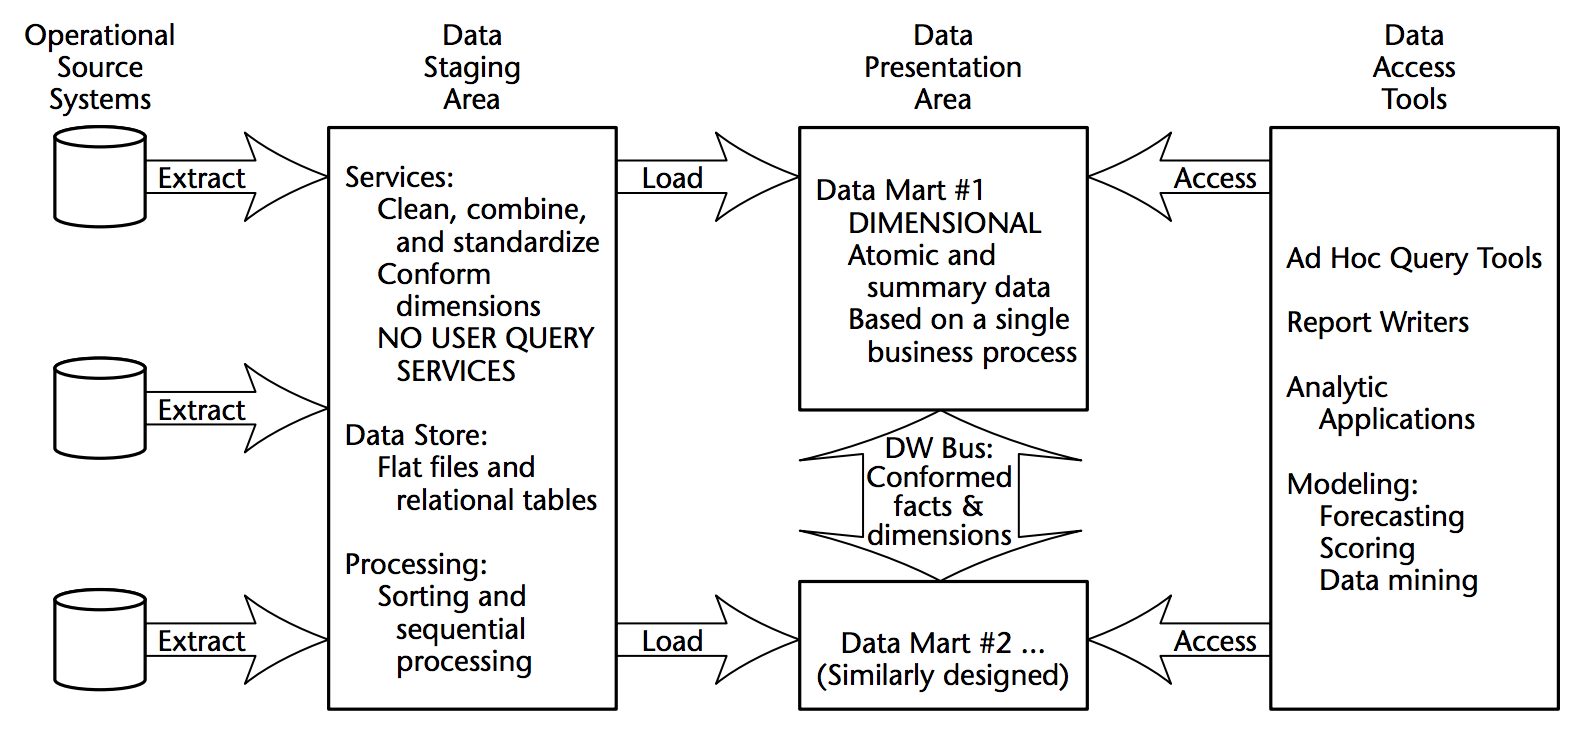
\includegraphics[width=.8\textwidth]{../elements_data_warehouse.png}
\caption{Elements of a Data Warehouse \cite{Kimball2011}}
\label{fig:figure1}
\end{figure}
 
The Data Presentation Area is where the data is organised, stored and accessed by analytical applications. According to 
\cite{Kimball2011}, this area should be composed by a series of integrated data marts, which are repositories that present the data for a single process of the organisational business. A data mart stores atomic data and organizes them in a model that is more legible to humans. The most popular technology used to implement data marts adopted by the industry is On-Line Analytical Processing (OLAP), that will be covered in more detail along this chapter. 

Finally, the Data Access Tools query the data in the presentation area. This element is formed by a set of different applications, since simple ad hoc queries until complex data mining application.

\section{Multidimensional Model}
The main functionality of a data warehouse is to facilitate multidimensional analysis \cite{OLAPCouncil}. This type of analysis reduces the number of misinterpretations by aligning the data with the analyst's mental model of the business. The multidimensional analysis provides an easy navigation through the database, showing specific subsets of data in different orientations and performing analytical calculations.
 
In order to perform multidimensional analysis, the data must be organised in a multidimensional model, where information is stored in a multidimensional array called \emph{hypercube} or \emph{cube} \cite{Vassiliadis1998}. A cube is composed by cells that store \emph{measures} aggregated by the data \emph{dimensions}. A \emph{dimension} is a cube's structural attribute formed by a list of properties that are similar to each other according to the user's perception of the data. Measures are the values being analysed by the user. Figure \ref{fig:figure2} shows an example of the dimensions and measures extracted from a sales application.
 
As shown in Figure \ref{fig:figure2} , each dimension (Geography, Time and Item) can be associated with an hierarchy of data aggregation levels. This feature allows user to view the data from different levels of details, for example: the measure \emph{Sales} aggregated by \emph{Region} can be detailed by \emph{Country} or even further detailed by \emph{City}.

\begin{figure}[ht]
\centering
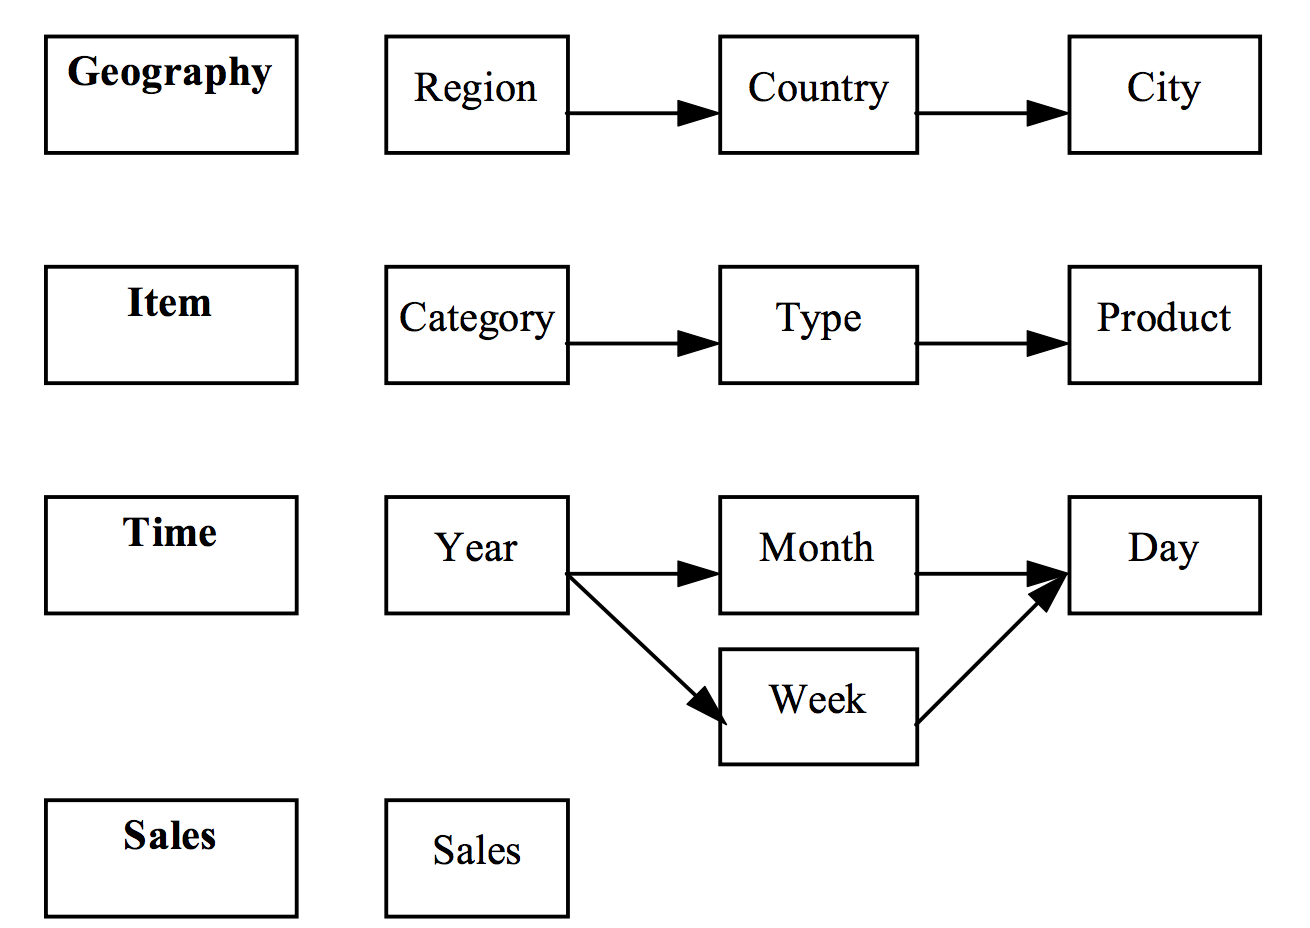
\includegraphics[width=.6\textwidth]{../dimensions_measures_example.png}
\caption{Example of dimensions and measure for a sales application  \cite{Vassiliadis1998}}
\label{fig:figure2}
\end{figure}

\section{OLAP}
On-Line Analytical Processing (OLAP) is a category of technological tools used by analysts and managers to extract new knowledge from consolidated enterprise data \cite{OLAPCouncil}. In order to achieve this goal, data are organised in cubes and stored following multidimensional models. The access to this data should be fast, consistent and interactive and it should provide various views of information, reflecting the different dimensions of an enterprise as perceived by the user.
 
Usually, the data loaded into an OLAP system comes from a data warehouse. According to \cite{Inmon2005}, the relationship between OLAP systems and data warehouse is complimentary: while OLAP offers control and flexible ways to explore data in different dimensions and hierarchy levels, data warehouse provides a robust data source for the OLAP system, where up-to-date data is available already extracted and properly integrated.

\subsection{Types of OLAP Systems}
There are two approaches for the physical model of an OLAP system \cite{Vassiliadis1999}: Multidimensional On-Line Analytical Processing (MOLAP) and Relational On-Line Analytical Processing (ROLAP) Architectures.The MOLAP architecture provides a direct multidimensional view of the data. This approach stores the data in a Multidimensional Database Management System (MDBMS), which use n-dimensional arrays that contains the measures of the cube. This type of DBMS has a better performance than traditional Relational Databases, but it is more difficult to manage updates.
 
The ROLAP architecture is a multidimensional interface to relational data. This approach uses a traditional Relational Database Management System (RDBMS) to store the data organised in a star or snowflake schema. A star schema is formed by one or more dimension tables and one centralised fact table, which stores the measures of interest for the OLAP system. Figure \ref{fig:figure3} shows an example of a star schema, where the tables TIME, GEOGRAPHY, ACCOUNT and PRODUCT are dimension tables and SALES is the fact table.

\begin{figure}[ht]
\centering
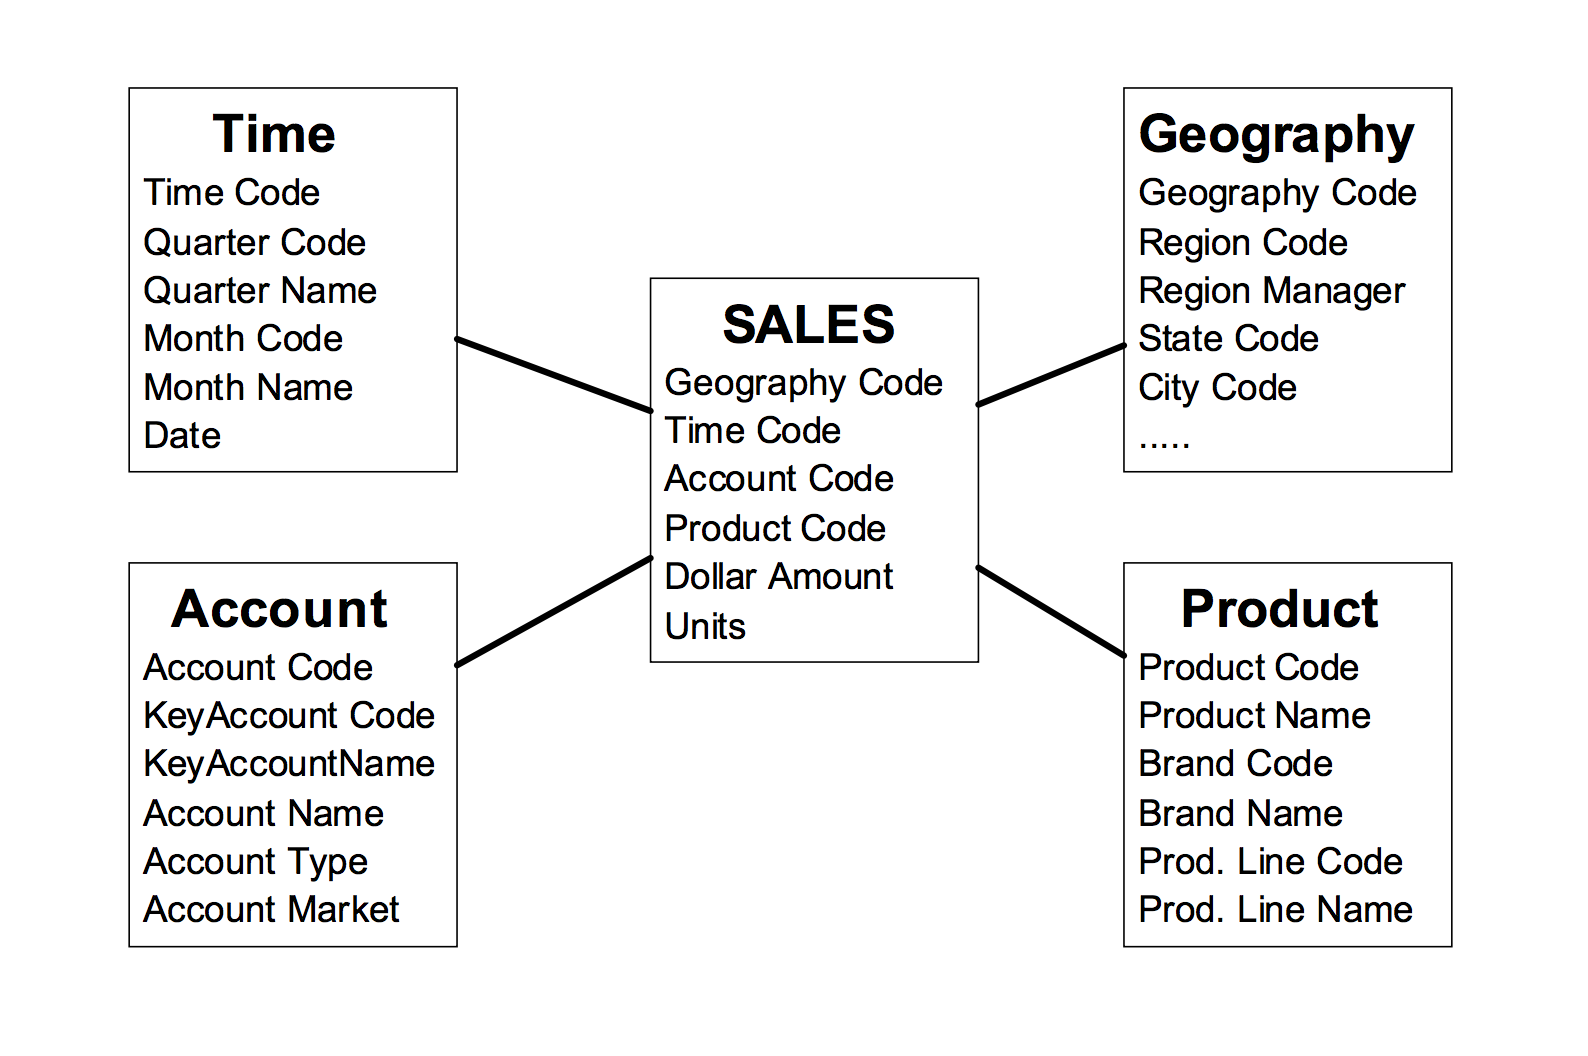
\includegraphics[width=.8\textwidth]{../star_schema_example.png}
\caption{Example of a Star Schema  \cite{Vassiliadis1999}}
\label{fig:figure3}
\end{figure}

Despite MOLAP architecture has the advantage of relying on a multidimensional native storage mechanism, the ROLAP approach allows easy integration with existing relational information systems and has the advantage of relational data being more efficiently stored than multidimensional data.

\subsection{OLAP Operators}
As mentioned earlier in this chapter, an OLAP system should provide a fast and interactive way for the user to explore the data stored in the cube. These are the main OLAP operations that can be used to navigate and manipulate different dimensions of the data \cite{Vassiliadis1998}:

\begin{description}
\item[Roll-up] Aggregates information along one dimension, summarising data on a higher level in its hierarchy. Consider the dimensions shown in Figure \ref{fig:figure2} and the measure of total dollar amount of sales per city, we can perform a roll-up operation to obtain the total dollar amount of sale per state.
\item[Drill-down] Detail information along one dimension, navigating the data from a higher to a lower hierarchy. Consider the measure of total dollar amount of sales per year, we can drill-down this query to obtain the total dollar amount of sales per month.
\item[Slice] Selects a slice of the cube according to user-specified dimension values. For instance, the user can select to view the total dollar amount of sales for the year of 2016.
\item[Dice] Selects a subcube from the original data according to user-specified conditions referred to more than one dimension. For instance, the user can select to view to total dollar amount of sales for the year of 2016 in the city of Recife.
\item[Pivot] Changes the orientation of dimensions in the cube, i.e. swap a row dimension to a column dimension.
\end{description}

There are other operations that can be performed in a OLAP system, but the ones shown above are considered the basic set of operations to support dynamic multidimensional analysis \cite{Inmon2005}.

\section{Graph}
Graph is a data structure formed by a set of vertices (or nodes) $V = \{v_1, \dots, v_n\}$  and a set of pair of vertices called edges (or relationships) $E = \{v_1v_2, \dots, v_nv_m\}$. It can be represented graphically (where the vertices are shown as circles and edges are shown as lines, as shown in Figure \ref{fig:figure4}) or mathematically in the form $G = (V, E)$ \cite{Tobergte2013}.

\begin{figure}[ht]
\centering
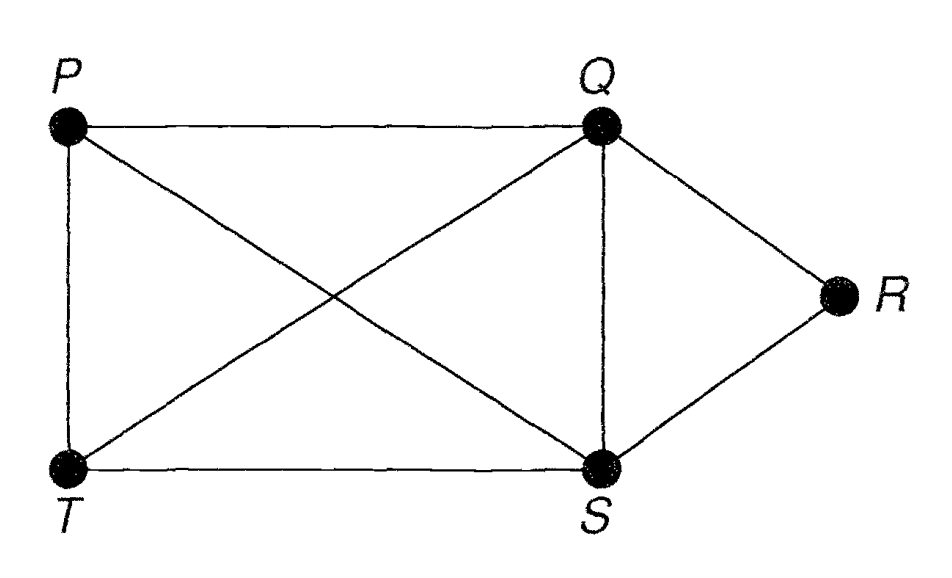
\includegraphics[width=.4\textwidth]{../graph_example.png}
\caption{Example of graph \cite{Tobergte2013}}
\label{fig:figure4}
\end{figure}

There are several real world applications that can take advantage of a graph model, specially the ones where the relationship between entities is an important information to be represented \cite{Miller2013}. Consider, for example, a social network application similar to Twitter, where a user can follow another user. In this scenario, we can represent a user as a vertex and the relationship between users as an edge, as shown in Figure \ref{fig:figure5}

\begin{figure}[ht]
\centering
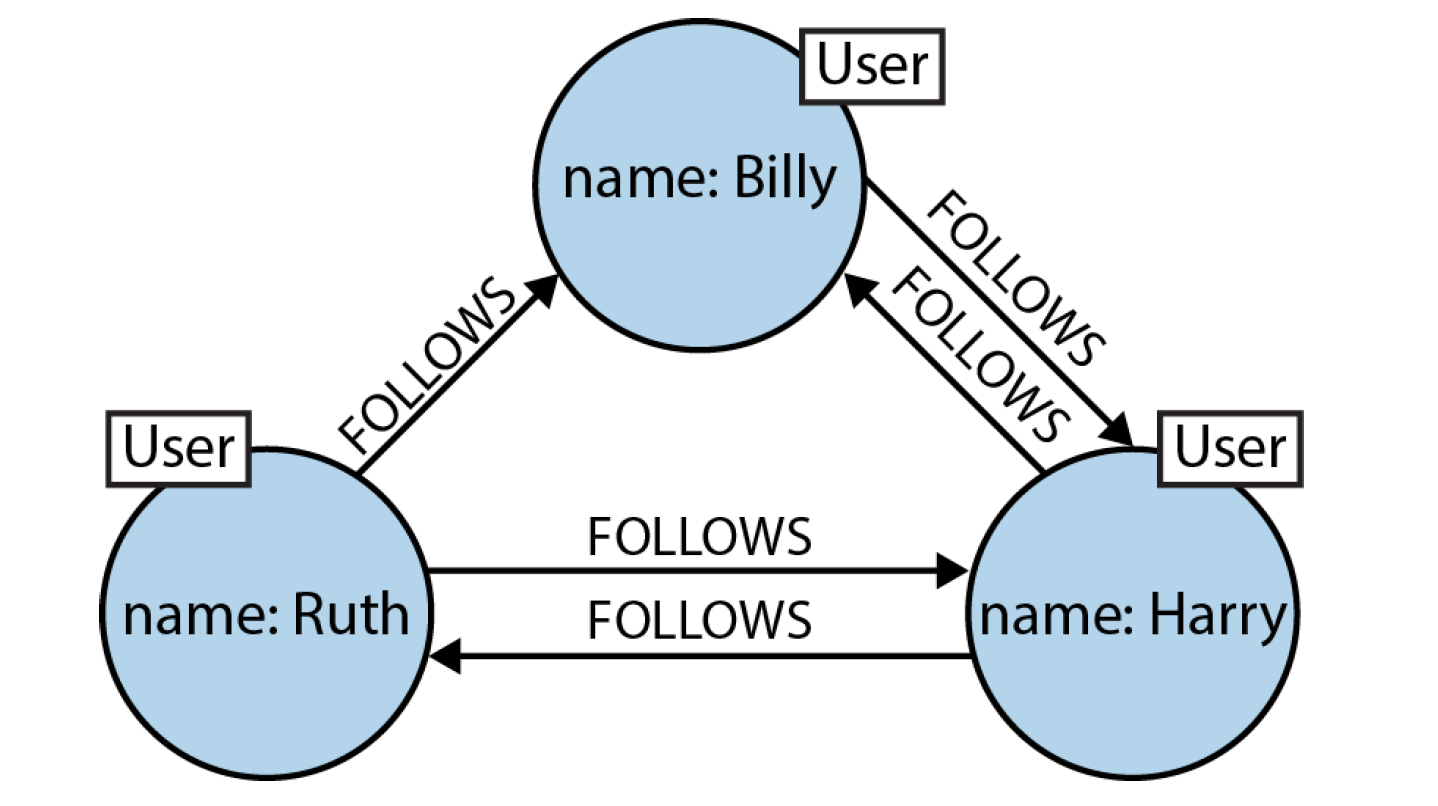
\includegraphics[width=.5\textwidth]{../social_network_graph_example.png}
\caption{Example of graph representation of a social network \cite{Miller2013}}
\label{fig:figure5}
\end{figure}

\subsection{Graph Theory}
Graph Theory is a branch of Mathematics dedicated to the study of graph structures \cite{Tobergte2013}. Given the definition of a general graph explained above, there are several classifications and concepts associated with graph structures.

\begin{description}
\item[Loop] When an edge starts and finishes in the same vertex, as the one shown in Figure \ref{fig:figure6} starting at vertex $T$ and finishing at vertex $T$.
\item[Multigraph] When a graph allows multiple edges connecting the same pair of vertices, as illustrated in Figure \ref{fig:figure6} with two edges connecting vertices $Q$ and $R$.

\begin{figure}[ht]
\centering
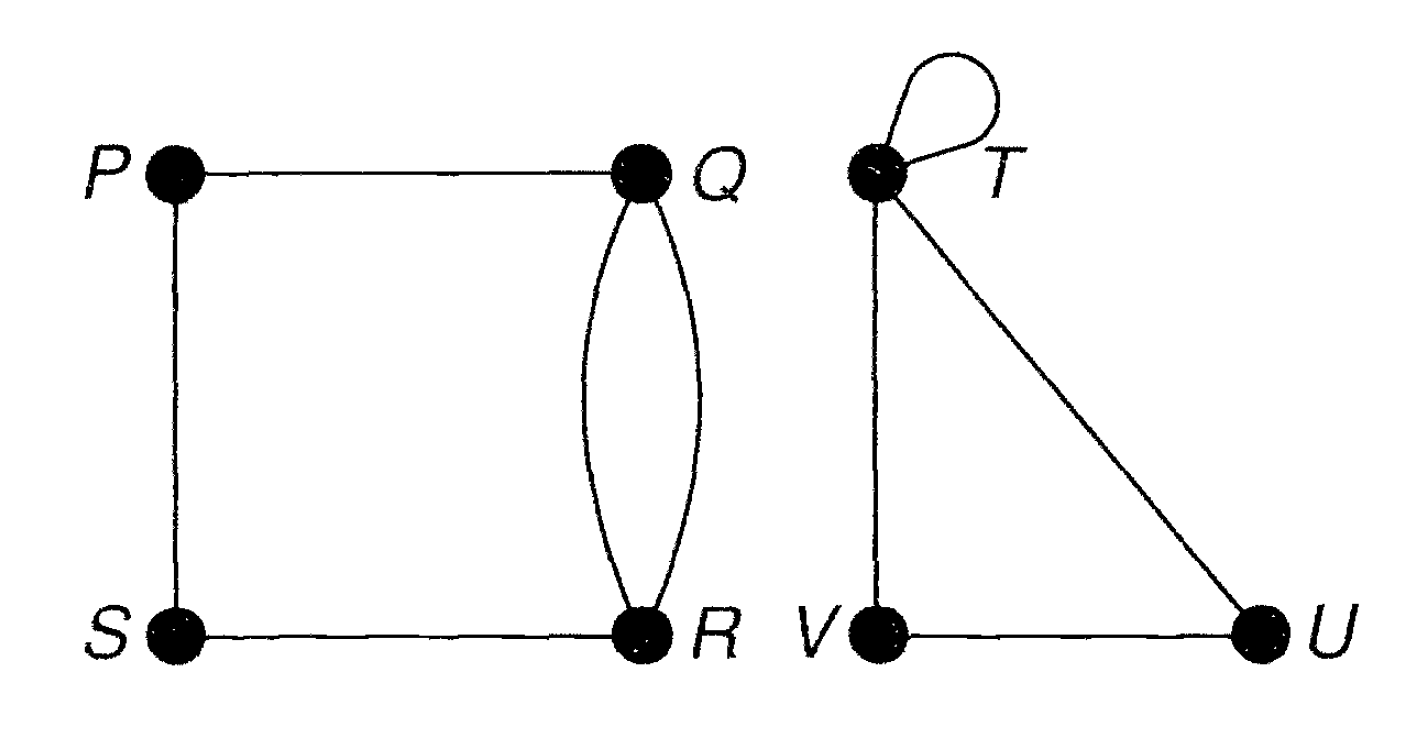
\includegraphics[width=.4\textwidth]{../loop_multigraph_example.png}
\caption{Example of a multigraph with a loop \cite{Tobergte2013}}
\label{fig:figure6}
\end{figure}

\item[Simple Graph] When a graph does not have loops or multiple edges, as the one depicted in Figure \ref{fig:figure4}.
\item[Complete Graph] When each pair of distinct vertices are connected to each other, as shown in Figure \ref{fig:figure7}.

\begin{figure}[ht]
\centering
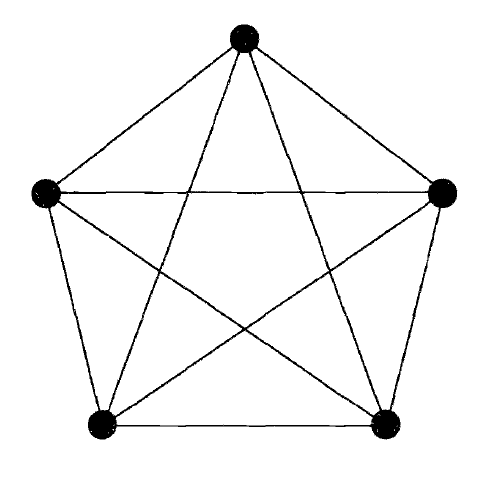
\includegraphics[width=.25\textwidth]{../complete_graph_example.png}
\caption{Example of a complete graph \cite{Tobergte2013}}
\label{fig:figure7}
\end{figure}

\item[Directed Graph] When the edges have directions expliciting the start and end of the connection, as illustrated in Figure \ref{fig:figure8}.

\begin{figure}[ht]
\centering
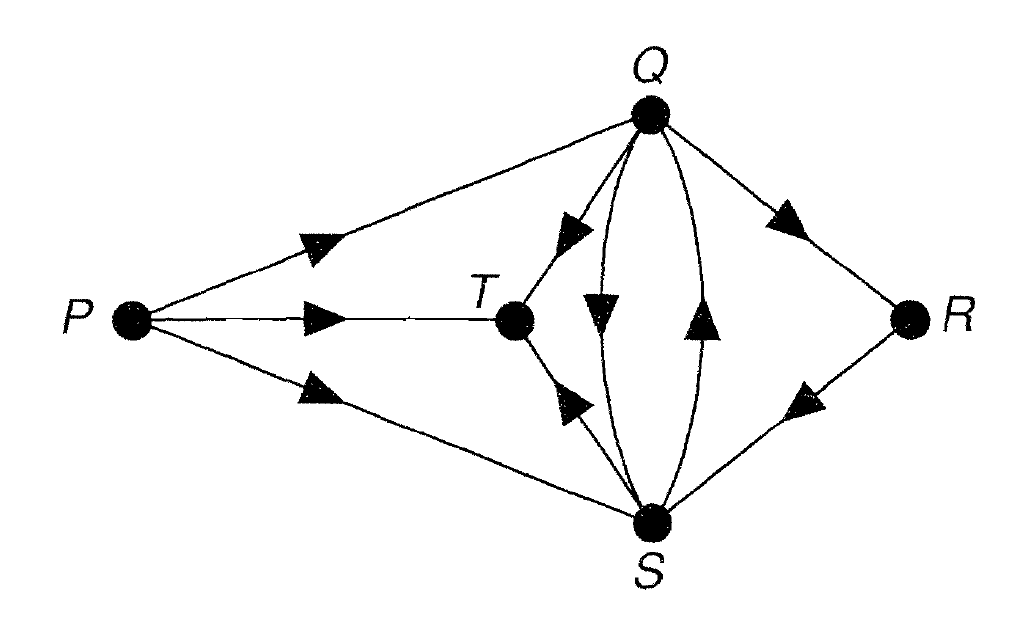
\includegraphics[width=.4\textwidth]{../directed_graph_example.png}
\caption{Example of a directed graph \cite{Tobergte2013}}
\label{fig:figure8}
\end{figure}

\item[Subgraph] It is a graph obtained from another graph $G$, where its vertices are a subset of the vertices of $G$ and its edges are a subset of the edges of $G$. Figure \ref{fig:figure9} shows in \ref{fig:figure9subfig2} a subgraph of the graph in \ref{fig:figure9subfig1}.
\item[Path] It is a subgraph obtained by a sequence of adjacent and distinct vertices.

\begin{figure}[ht]
\centering
\begin{subfigure}{.4\textwidth}
	\centering
	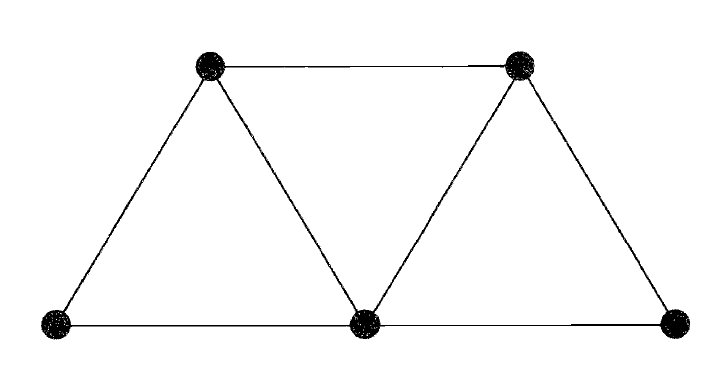
\includegraphics[width=.5\textwidth]{../subgraph_example_1.png}
	\caption{Original graph}
	\label{fig:figure9subfig1}
\end{subfigure} %
\begin{subfigure} {.4\textwidth}
	\centering
	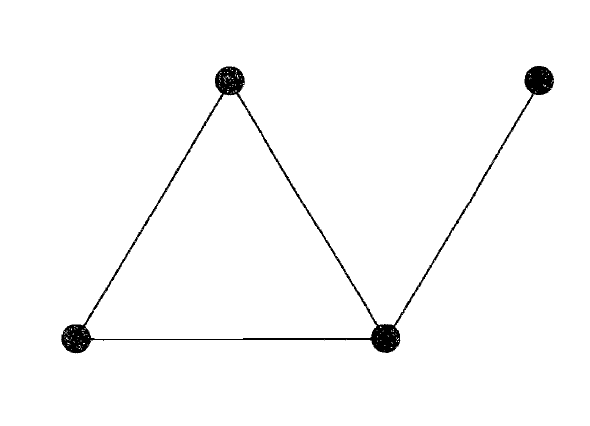
\includegraphics[width=.5\textwidth]{../subgraph_example_2.png}
	\caption{Subgraph}
	\label{fig:figure9subfig2}
\end{subfigure}
\caption{Example of a subgraph \cite{Tobergte2013}}
\label{fig:figure9}
\end{figure}
\end{description}
There are other types of classifications of a graph and other concepts associated to it \cite{Tobergte2013}. These are the main definitions for the purposes of understanding the work presented here.

\subsection{Network Analysis}

There are different kind of analysis that can be done depending on the nature of the graph data. Due to the work presented here, we will explore the aspects of social network analysis, which focus on the structure of relationships (edges) between entities (vertices) in the graph. Several types of analysis can be performed in a graph, but the measure of a node's centrality is historically one of the most studied cases of analysis \cite{Freeman1978}. A common application for a centrality measure is to find out what are the focal points in a social network, i.e. who are the people that are the most connected to other people? There are three types of centrality measures \cite{Freeman1978}:

\begin{description}
\item[Degree Centrality] This measure is given by the number of adjacent vertices. Considering a social network, a person (vertex) that has the greatest number of connections can be considered one of the focal points of the network, since it can directly read the most nodes in the graph. Given a graph with n vertices, the maximum value the degree centrality of a vertex in the graph can be is $n-1$. The degree centrality of a vertex is related to its potential communication activity.

\item[Betweenness Centrality] This measure is given by the frequency in which a vertex is present in the shortest path between other vertices. Considering a social network, a person with high betweenness centrality is capable of influencing others by intercepting connections between several vertices in the graph. The betweenness centrality of a vertex is related to its potential control of communication.

\item[Closeness Centrality] This measure is given by the inverse of the average distance of the shortest path of a vertex between other vertices in the graph. Considering a social network, a person with high closeness centrality do not depend as much on others to communicate with other people in the network. The closeness centrality of a vertex is related to its potential independency and efficiency to control communication.
\end{description}

\section{Graph Databases}

Graph Databases are an alternative to Relational Database Management Systems (RDBMS), which are commonly used in the industry since the early 1980's. Despite the popularity of RDBMSs, GDBs allow the storage of data in graph model, which is a more natural way to represent information for some applications, such as social networks, semantic web pages and recommendation systems \cite{Miller2013}. 

The most popular form of graph model is the labeled property graph model \cite{Robinson2015}. The main characteristics of a labeled property graph are:
\begin{itemize}
\item Nodes (vertices) and Relationships (edges) can contain properties, i.e. key-value pairs
\item Nodes can be labeled with one or more labels
\item Relationships are named and directed, i.e. always have start and end nodes
\end{itemize}

The formal definition for a labeled property graph is given by $G = (V, E, L_V, L_E, A_V, A_E)$, where:
\begin{itemize}
\item $V$ is a set of vertices (nodes)
\item $E \subseteq V \times V$ is a set of edges 
\item $L_V$ is a set of node labels and $L_E$ is a set of edge labels
\item $A_V = \{a_1, \dots, a_n\}$ is a set of node attributes, where $a_i = (k_i, m_i)$ is a key-value pair. Each vertex $v_i \in V$ is associated with an attribute vector. $A_E = \{b_1, \dots, b_n\}$ is the set of edge attributes defined in the same way as node attributes.
\end{itemize}

An example of a labeled property graph was shown in Figure \ref{fig:figure5}, where the nodes have the label ``User'' and the property ``name'' and the relationships are named ``Follows'' and have arrows indicating the direction of the edge.

\subsection{Historical Overview}

Scientific research related to graph data models were continuously published between 1980's and the first half of 1990's. Then, the database community attention turned to semistructured data model, due to the emergence of XML and the growth of hypertext document applications \cite{Angles2008}. From this period, the main focus of the graph databases proposed was to establish a better way to represent data and methods to retrieve and manipulate data modeled as graph.
 
Recently this area has gained again attention from the community, due to the emergence of trendy projects (chemistry, biology, social network, semantic web, among others) where the importance of information relies not only in the entities but also in the relationship between them \cite{Angles2012}. Most recent implementations of graph databases are concerned with handling increasing amount of data and improving performance in retrieving and manipulating data.
 
The most popular graph database according to DBEngines\footnote{https://db-engines.com/en/system/Neo4j} website is Neo4J\footnote{https://neo4j.com/}. It is an open source native graph storage database implemented in Java. Neo4J has its own query language called Cypher, which can be used to create, update and retrieve nodes and relationships. This graph database also provides high availability and scalability for big volume of graph data.

Besides Neo4J, there are other popular graph databases according to DB Engine site. OrientDB\footnote{http://orientdb.com/orientdb/} is a NoSQL Multi-Model database, which means it stores data in the form of documents, key-value stores, objects, graph and others. Like Neo4J, OrientDB is also implemented in Java, but it uses an extended version of SQL that includes special operators to manipulate graph. This database allows the creation of a pre-defined data schema and the definition of complex data type, like dates, decimals and binary objects (BLOB).
 
TitanDB\footnote{http://titan.thinkaurelius.com/} is a native graph database implemented in Java. In order to establish connection with the hard disk, Titan needs to be linked to a data storage system - Cassandra\footnote{http://cassandra.apache.org/}, HBase\footnote{https://hbase.apache.org/} or BerkeleyDB\footnote{http://www.oracle.com/technetwork/database/database-technologies/berkeleydb/overview/index.html} - that is suitable for the application. The creation of nodes, edges and the submission of queries can be done through a Java API or through a Gremlin server.

\subsection{Comparing Graph Databases Performance}
One of the basic tasks when manipulating a database is to retrieve an object given its id. The experiment described in \cite{jouili2013empirical} records the average time to retrieve a node by its id, given an 500000 nodes graph and 4 clients executing this action 200 times. This process was executed using Neo4J, OrientDB and TitanDB using Cassandra as backend.

\begin{figure}ht]
\centering
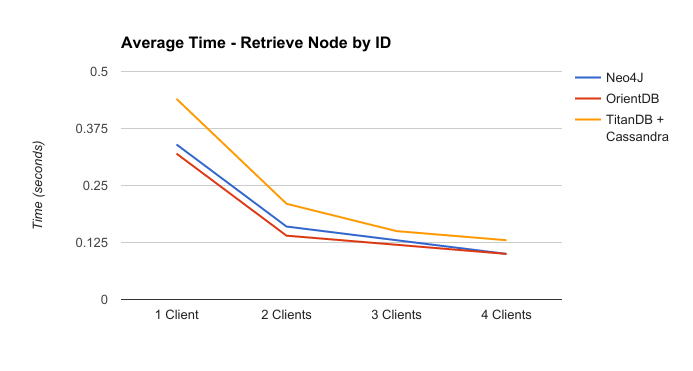
\includegraphics[width=1\textwidth]{../time_test.png}
\caption{Chart with mean time that each DB took to retrieve a node by its id}
\label{fig:figure10}
\end{figure}

According to Figure \ref{fig:figure10}, Neo4J and OrientDB have similar performance, being OrientDB slightly faster to retrieve a node given its id. On the other hand, TitanDB using Cassandra as backend has a bad performance compared with the other DBs. However, TitanDB can be connected with other backend services, which can improve its performance for this task.
 
Another common concern among developers is the amount of memory taken by the database. In the experiment shown in \cite{mccoll2014performance}, a graph containing 32,000 nodes and 256,000 edges was stored in Neo4J, OrientDB and TitanDB and the amount of memory required by each database was measured.

\begin{figure}[ht]
\centering
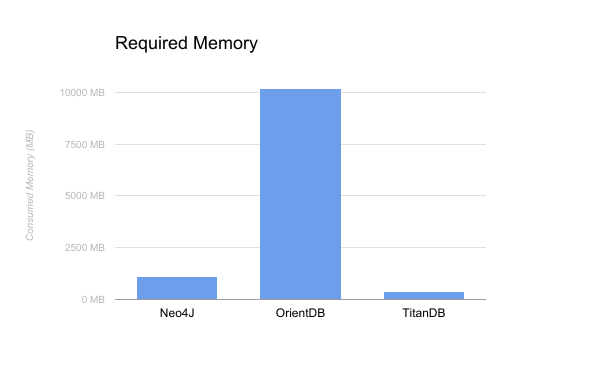
\includegraphics[width=1\textwidth]{../memory_test.png}
\caption{Chart with the amount of memory required for each DB}
\label{fig:figure11}
\end{figure}

From the Figure \ref{fig:figure11}, we can notice that OrientDB is the one that consumes the most, reaching up to 10.156 MB of memory. On the other hand, TitanDB requires less memory, only needing 388 MB to store the graph.

\section{Final Considerations}
In this chapter, we discussed the main concepts related to the work presented in this dissertation. Initially, the definition of Data Warehouse and Multidimensional Model were introduced, followed by a detailed view on different types and operators an OLAP system can have. Then, we covered the main components of a graph and how it can be classified according to different characteristics. Finally, we explained the definition of a Graph Database and went through a historical overview of such systems, as well as a comparison of the most popular Graph DBs nowadays. In the next chapter, we will review the most important research published that implements a OLAP system using Graph Databases.

% ---
% Literature Revision
% ---
\chapter{Graph Cubes: State of the Art}
% ---

This chapter presents the most important research works published in the area of OLAP systems implemented using graph databases. The first work presented here dates back to 2011 and introduces several concepts - such as graph cube, aggregated graphs and cuboid queries - that serve as basis for other papers published since then.

\section{Graph Cube: On Warehousing and OLAP Multidimensional Networks}

One of the main works in graph analysis using OLAP methods is described in \cite{Zhao2011}, and it  introduces several concepts that will be used by other authors to describe their work in this area. Graph Cube is one of those concepts and it is defined as a multidimensional model that extends multidimensional networks to provide decision support features. A multidimensional network is a graph $N=(V,E,A)$, where $V$ is a set of vertices, $E$ is a set of edges and $A$ is a set of vertex-specific attributes. Each vertex in the graph is a multidimensional tuple and the attributes of the vertex define the graph cube dimensions.
 
A graph cube is formed by all possible aggregate networks calculated from the original multidimensional network. An aggregate network (often called cuboid) is a summarisation of the original graph with respect to one or more dimensions, which is calculated by applying an aggregate function (e.g. COUNT, SUM, AVERAGE, among others) on the vertices attributes. Consider the multidimensional network illustrated in Figure \ref{fig:figure12}.

\begin{figure}[ht]
\centering
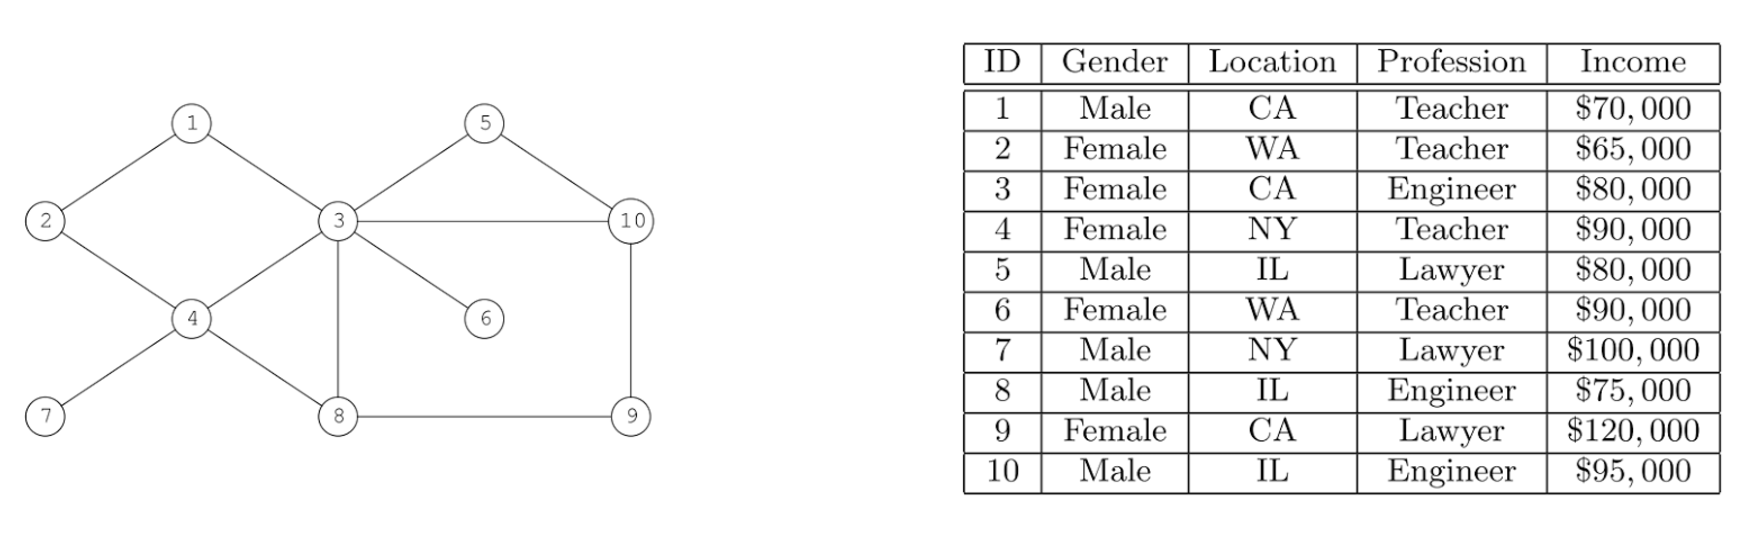
\includegraphics[width=1\textwidth]{../multidimensional_graph.png}
\caption{Multidimensional network \cite{Zhao2011}}
\label{fig:figure12}
\end{figure}

\begin{figure}[ht]
\centering
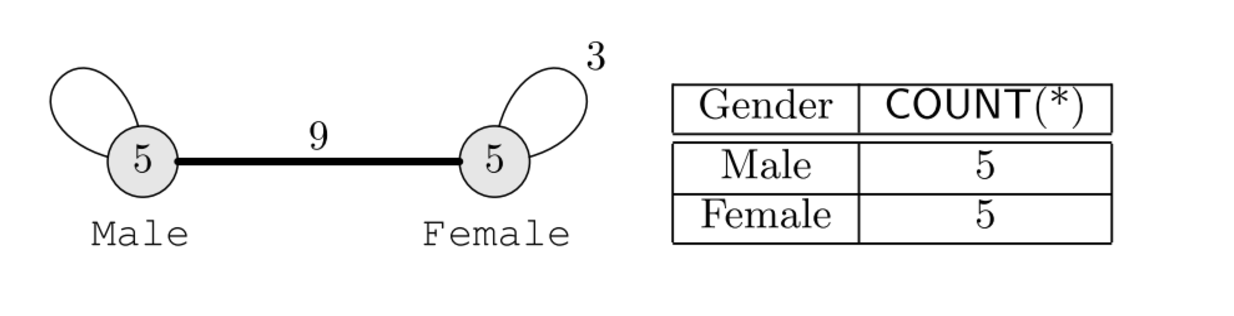
\includegraphics[width=0.8\textwidth]{../aggregate_graph.png}
\caption{Aggregate Network by \emph{Gender} dimension \cite{Zhao2011}}
\label{fig:figure13}
\end{figure}

The vertices of the graph presented in Figure \ref{fig:figure12} represent individuals and the edges represent the relationship between these individuals. The table on the right side of Figure \ref{fig:figure12} describes the attributes of each vertex: an unique \emph{ID}, \emph{Gender}, \emph{Location}, \emph{Profession} and \emph{Income}. Figure \ref{fig:figure13} shows the cuboid obtained by applying the function COUNT on the attribute \emph{Gender}: two nodes represent the possible values for the attribute (Male and Female) and they contain the number of nodes in the original graph with the respective \emph{Gender} value. It is important to notice that the relationship between individuals was also aggregated in the resulting network, e.g. the aggregate network show that there are 9 relationships between male and female individuals in the original graph.

The dimension of a cuboid is given by the set of non-aggregate dimensions of the cuboid. For instance, the cuboid in Figure \ref{fig:figure13} has the dimension \emph{Gender}. A cuboid $A'$ is an ancestor of another cuboid $A''$ if $dim(A')$ contains $dim(A'')$. Given these definitions, all possible cuboids of a graph cube can be organised in a graph cube lattice, ordering the cuboids according to its ancestors. A multidimensional network $N$ with $n$ dimensions has $2^n$ cuboids in the graph cube. Figure 3 shows the graph cube lattice for the multidimensional network introduced in Figure \ref{fig:figure12}, considering only \emph{Gender}, \emph{Location} and \emph{Profession} as dimensions.

\begin{figure}[ht]
\centering
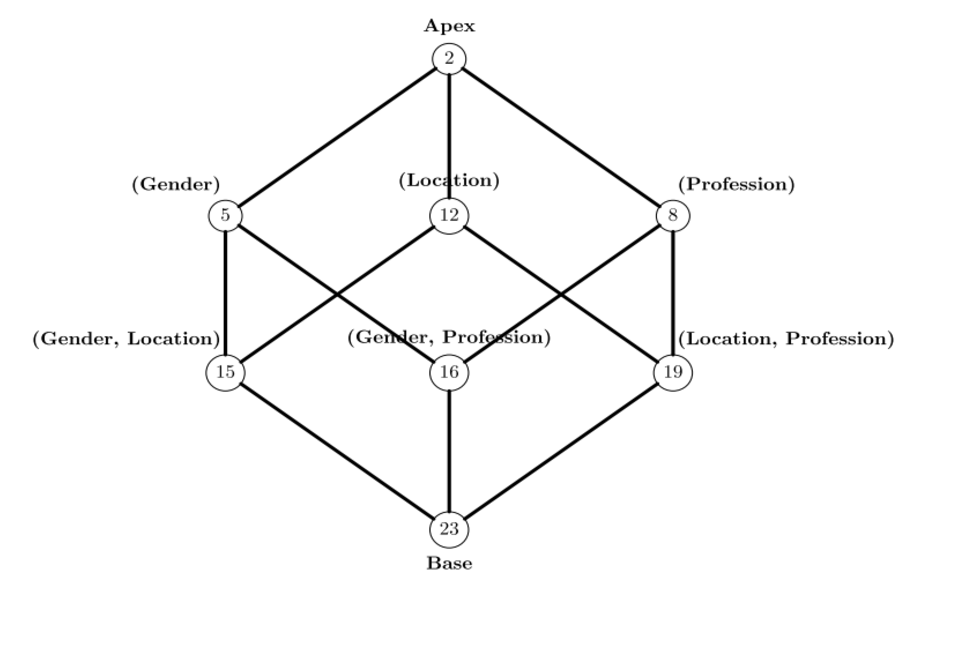
\includegraphics[width=0.6\textwidth]{../graph_lattice.png}
\caption{Graph Cube Lattice \cite{Zhao2011}}
\label{fig:figure14}
\end{figure}

The paper proposes two OLAP query models:
\begin{description}
\item[Cuboid Query] Aggregate vertices and edges based on the dimension requested in the query and can work with any aggregate function (SUM, AVG, etc). For instance, consider a graph with nodes containing the attributes (\emph{Gender}, \emph{Location}, \emph{Profession}). A cuboid query for this graph can be (\emph{Gender}, *, *) which will result in an aggregate graph showing all the vertices with the same Gender value aggregated and the edges also aggregate by the function COUNT.
\item[Crossboid Query] Returns the aggregate network between two or more cuboids structures. An example of a crossboid query can be the aggregate network between an user with $ID = 3$ and all the locations
\end{description}

Given that the size of the graph cube lattice is exponential with respect to the number of dimensions of the original multidimensional network, the paper proposes a partial materialisation in order to process queries. The partial materialisation is implemented using a greedy algorithm that selects $k$ cuboids $(k < 2^n)$ to be materialised according to the benefit of those cuboids to improve the cost for query evaluation.
 
The graph cube implementation described above is also studied by other works. In \cite{Denis2013}, a distributive approach is proposed using map reduce jobs to calculate each step of the aggregation process. In \cite{Khan2014}, a new algorithm to compute the Graph Cube (iGraphCubing) is proposed, using a new prunning method based on the Structural Significance measure.This measure takes into account three factors:
\begin{itemize}
\item The diversity of the attribute value in the neighborhood for each vertex
\item The clustering coefficient
\item The density around each vertex
\end{itemize}
 
The work in \cite{Zhao2011} presents experiments evaluating the effectiveness and the efficiency of the method proposed. The effectiveness was evaluated by analysing OLAP queries submitted to the graph cube. The efficiency was evaluated by analysing the graph cube performance depending if it was fully or partially materialised in disk. In conclusion, the paper proposes an implementation of a graph cube obtained from an homogeneous attributed graph, but it does not consider heterogeneous networks neither attributed edges

\section{Graph OLAP: Towards Online Analytical Processing on Graphs}
The Graph OLAP framework  proposed in \cite{Chen2008} takes as input a set of network snapshots, where each snapshot contains a graph and a set of informational attributes that describes the snapshot. In this scenario, the paper defines two dimension types: informational dimensions (formed by the informational attributes) and topological dimensions (formed by the attributes of the nodes and edges of the graph). The authors distinguish different semantics for OLAP operations in graphs, so these operations are categorised into Informational OLAP (I-OLAP) and Topological OLAP (T-OLAP). 
 
The framework gives as output an aggregate graph with a summarised view of the snapshots set. The type of the aggregate graph returned by the framework can also be categorised in Informational Aggregate Graph (I-aggregate graph) and Topological Aggregate Graph (T-aggregate graph). 
 
Informational Aggregate Graph is computed based on a set of network snapshots that have informational dimensions with same values. Figure \ref{fig:figure15} shows an example of an i-aggregate graph composed by snapshots describing the co-author relationship between individual authors. The co-author relationship is grouped by a certain conference (\emph{sigmod}, \emph{vldb}, \emph{icde}), by a class of conferences (\emph{db-conf}), by a specific period of time (\emph{2004}, \emph{2005}) and by a group of time periods (\emph{all-years}). It is important to notice that the graph in Figure \ref{fig:figure15} shows different levels of aggregations for each co-author relationship. 

\begin{figure}[ht]
\centering
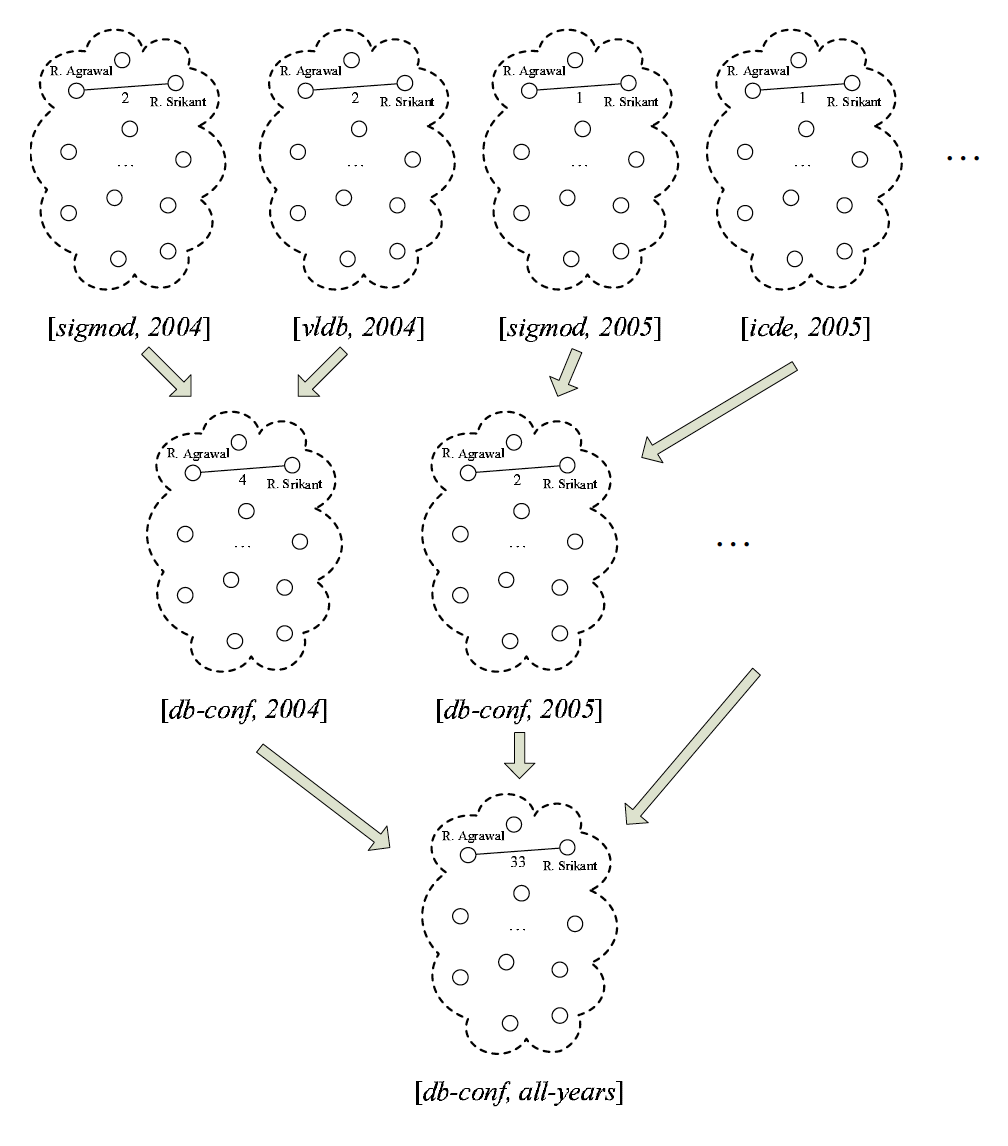
\includegraphics[width=0.6\textwidth]{../i_aggregated_graph_example.png}
\caption{Example of Informational Aggregate Graph \cite{Chen2008}}
\label{fig:figure15}
\end{figure}

Classic OLAP operations in an i-aggregate graph can be interpreted as follows:
\begin{description}
\item[Roll-up] Aggregate multiple snapshots to form a higher level summary of information
\item[Drill-down] Return to lower-level snapshots from aggregate graph
\item[Slice / dice] Select a subset of snapshots based on informational dimensions
\end{description}
 
Topological Aggregate Graph is obtained based on a single network, where the nodes are the result of applying the aggregate function to the nodes of the original network with the same attribute value. Figure \ref{fig:figure16} shows an example of a t-aggregate graph where the information about co-author relationship between individual authors in one snapshot was aggregated into co-author relationship between the institutions the authors belong to.

\begin{figure}[ht]
\centering
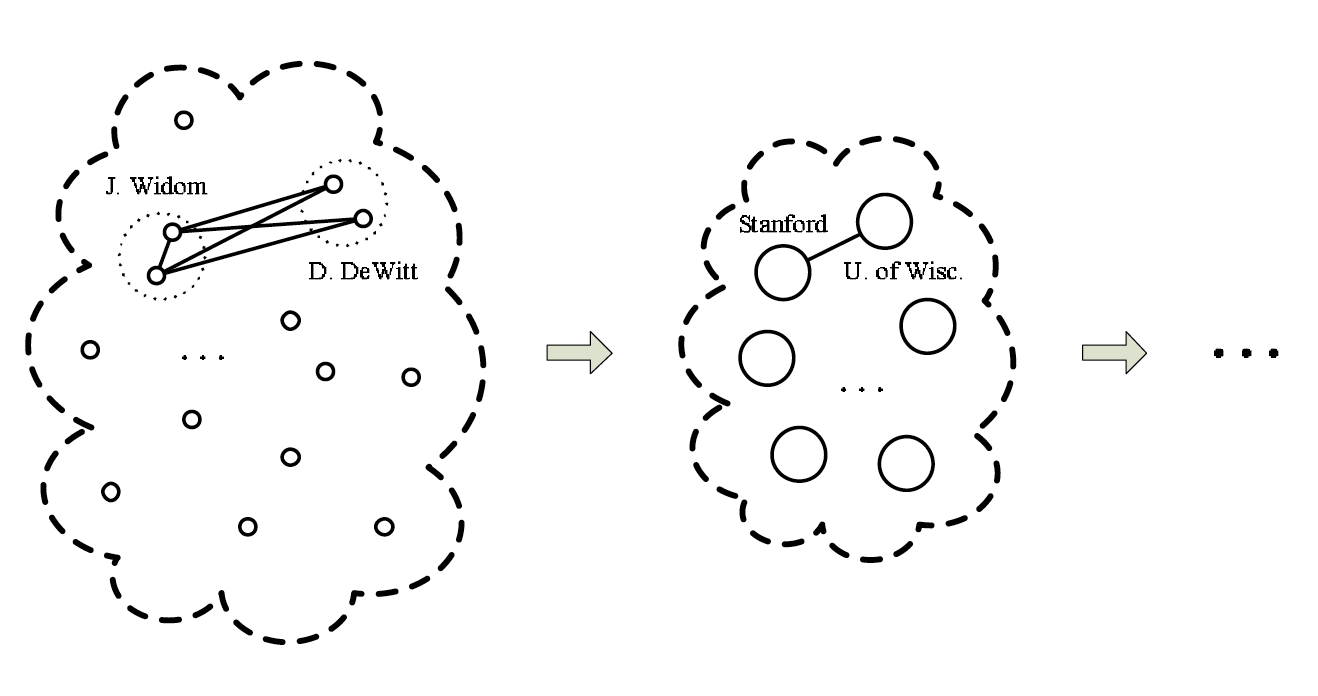
\includegraphics[width=0.7\textwidth]{../t_aggregated_graph_example.png}
\caption{Example of Topological Aggregate Graph \cite{Chen2008}}
\label{fig:figure16}
\end{figure}

Classic OLAP operations in an t-aggregate graph can be interpreted as follows:
\begin{description}
\item[Roll-up] Merge topological elements (nodes or edges) and replace them by corresponding higher-level elements
\item[Drill-down] Split merged elements into lower-level elements
\item[Slice / dice] Select a subgraph of a snapshot based on topological dimensions
\end{description}

The Topological OLAP is further explained in \cite{Qu2011}. This work takes into consideration two properties (T-Distributiveness and T-Monotonicity) used to classify how different measures can be performed in an OLAP Graph. A measure function is considered T-Distributive if the result of the function applied to high-level nodes from the graph can be obtained by the computation of pre-computed results of the same function applied to lower-level nodes from the same graph. On the other hand, a measure is considered T-Monotone, if the data search space can be pruned given a user-defined threshold, by dropping node pairs with measures that don't satisfy the threshold. The paper shows experiments using common constraint function, proven to be T-Distributives and/or T-Monotones, such as SUM, MIN, MAX, Density, Degree Centrality, Closeness Centrality, among others.

\section{HMGraph}
An Heterogeneous and Multidimensional Graph OLAP framework (HMGraph OLAP) is proposed in \cite{Yin2012}. This framework uses a graph model similar to Graph OLAP \cite{Chen2008}, but it adds the concept of Entity Dimensions due to the heterogeneity of the input graphs (Graph OLAP framework only handles homogeneous graphs). Figure \ref{fig:figure17} shows an example of a heterogeneous multidimensional network, highlighting the entity attributes of the graph.

\begin{figure}[ht]
\centering
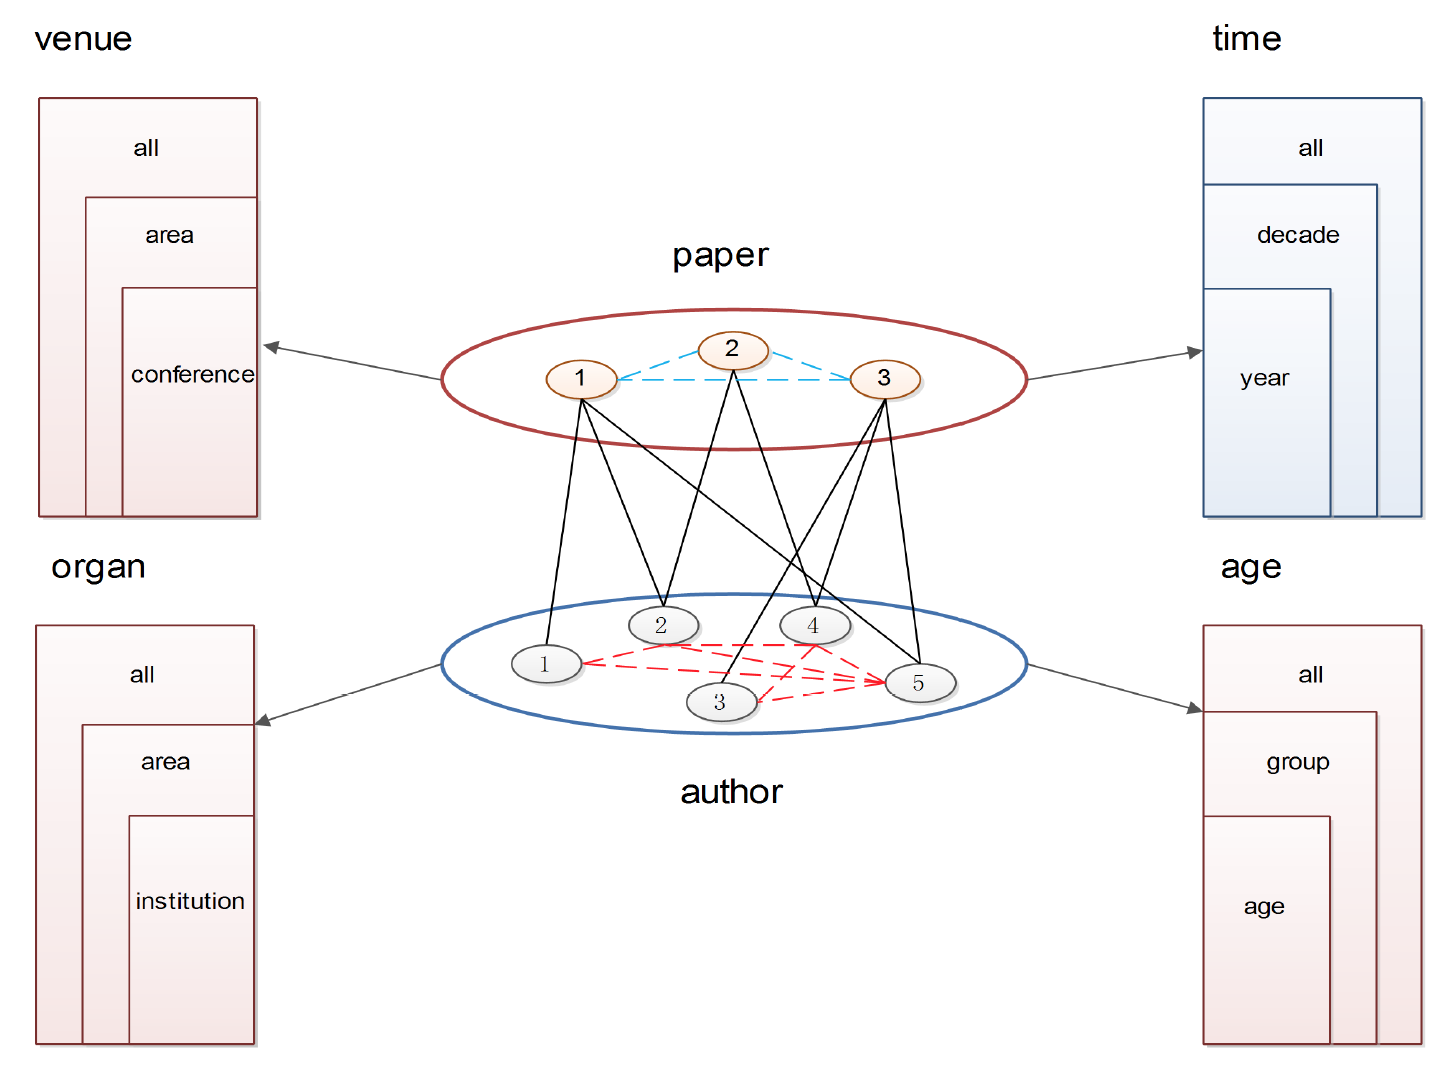
\includegraphics[width=0.7\textwidth]{../heterogeneous_graph_example.png}
\caption{Example of a heterogeneous multidimensional network \cite{Yin2012}}
\label{fig:figure17}
\end{figure}

Entity attributes are the attributes that describe the characteristics of an entity. In the graph illustrated in Figure \ref{fig:figure17}, organ and age are entity attributes of author entity. Entity Dimension is related to the types of nodes in the graph.

Like Graph OLAP, HMGraph can perform I-OLAP and T-OLAP operations, but it can also perform rotate and stretch operations. The rotate operation is done by changing nodes into edges and edges into nodes, as shown in Figure \ref{fig:figure18}. The stretch operation is done by changing edges into entities and adding edges between the recently created entity and the nodes previously connected to the transformed edge, as shown in Figure \ref{fig:figure19}.

\begin{figure}[ht]
\centering
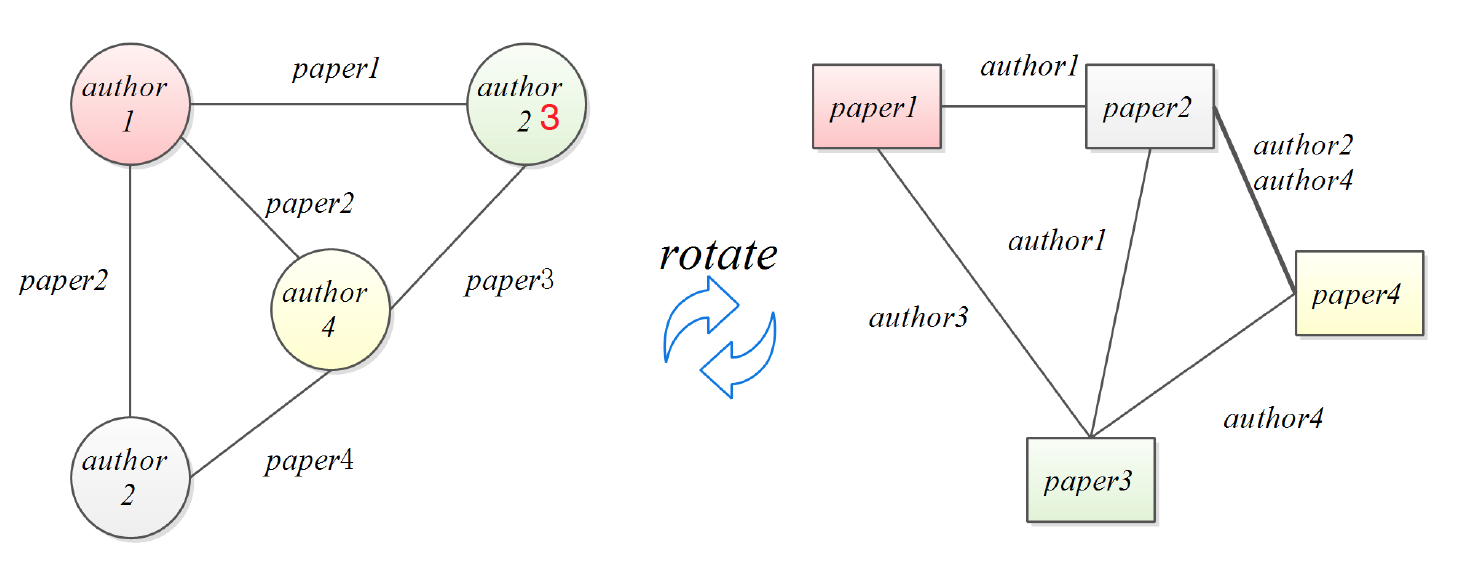
\includegraphics[width=0.7\textwidth]{../rotate_operation_example.png}
\caption{Example of rotate operation \cite{Yin2012}}
\label{fig:figure18}
\end{figure}

\begin{figure}[ht]
\centering
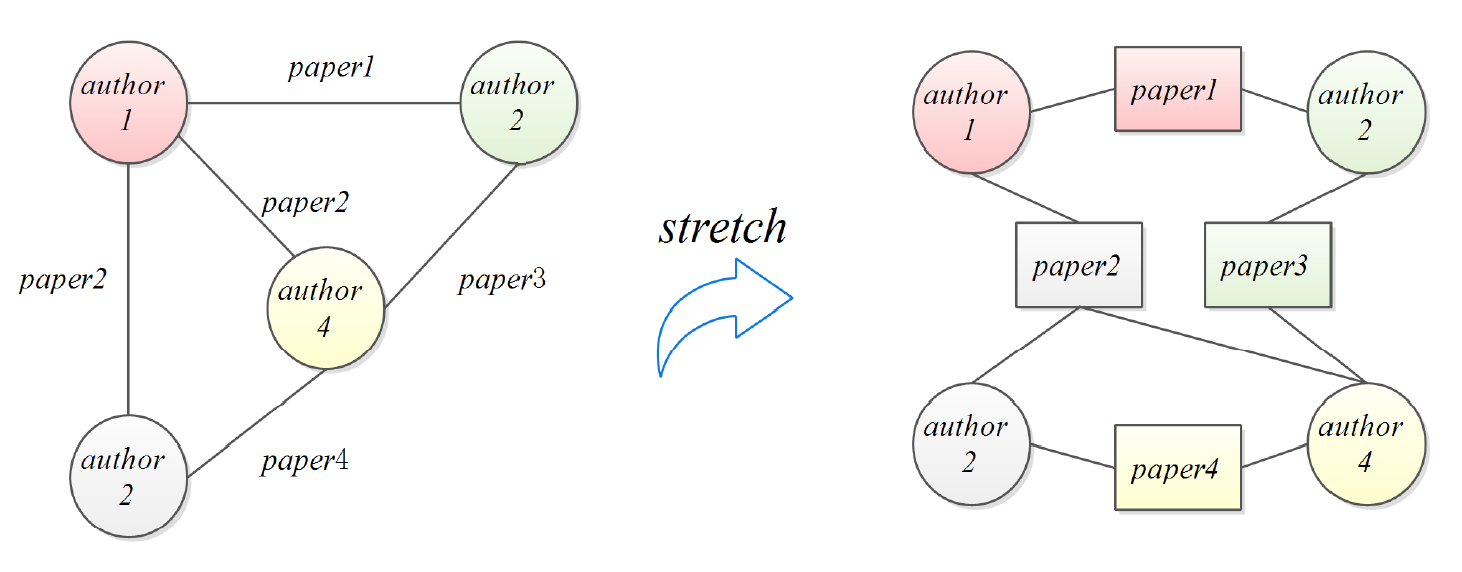
\includegraphics[width=0.7\textwidth]{../stretch_operation_example.png}
\caption{Example of stretch operation \cite{Yin2012}}
\label{fig:figure19}
\end{figure}

Even though the work presented in \cite{Yin2012} draws attention to the importance of heterogeneous networks in real world application, the paper does not provide further implementation detail on how the framework can be used with real data.

\section{Pagrol: PArallel GRaph OLap over Large-scale Attributed Graphs}

The work presented in \cite{Wang2014} proposes a parallel Graph OLAP system, adopting the Hyper Graph Cube model that extends attributed graphs to support decision making services. The model proposed in this paper is similar to the Graph Cube described in \cite{Zhao2011}, with the main difference being the presence of attributes also in the graph edges. In this scenario, there are two types of dimensions: vertex dimensions and edge dimensions. Figure \ref{fig:figure20} shows an example of an attributed graph.

\begin{figure}[ht]
\centering
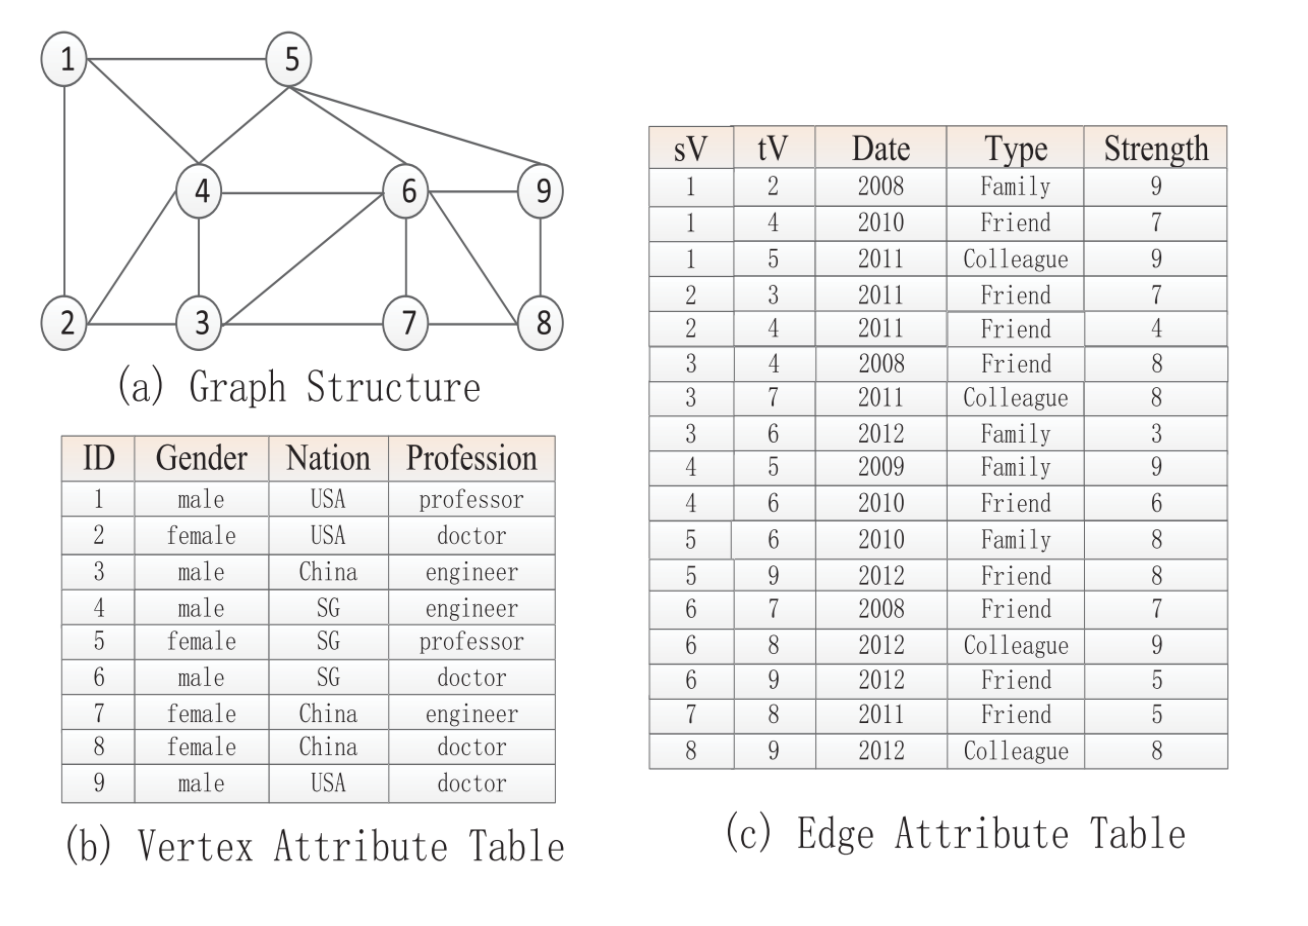
\includegraphics[width=0.8\textwidth]{../attributed_graph.png}
\caption{Example of attributed graph \cite{Wang2014}}
\label{fig:figure20}
\end{figure}

Given an attributed graph with n vertex dimensions and m edge dimensions, the Hyper Graph Cube will contain $2^{n+m}$ aggregate graph obtained as described by the work of \cite{Zhao2011}. This Hyper Graph Cube can be seen as the cartesian product between all the vertex-aggregate networks (when one or more vertex dimensions are aggregated ) and the edge-aggregate networks (when one or more edge dimensions are aggregated). This cube arrangement can support the following query categories:
\begin{description}
\item[Category 1] Queries answered by information stored either in a vertex or  in a edge attributes. For example:``How many relationships appeared in 2012?'' or ``What is the percentage of users in each different professions in this network?''
\item[Category 2] Queries answered by integrating the knowledge stored in both vertex and edges attributes. For example: ``What is the trend of the number of relations appearing between USA and SG (Singapore) in the last 3 years?''
\item[Category 3] Queries answered by an aggregate graph, that provides a summarised view of the data along some dimensions. For example: ``What is the graph structure as grouped by users' gender as well as relationship type?''
\end{description}

The Hyper Graph Cube also supports roll-up and drill-down operations, along both vertex and edge dimensions. For instance, if we have an aggregate graph along Location dimension according to City value, we can roll up to obtain an aggregate graph according to State value.
 
The materialisation for the Hyper Graph Cube is done using Map-Reduce (MR) jobs. Since vertex and edges are stored in two different tables in the distributed file system (DFS), the materialisation is done in two steps: first the two tables are joined into one flat table containing all the dimensions and the second step performs the cube computation. This process is optimised using self-contained joins and batching techniques.

\section{GRAD Graph Cubes}

One of the most recent works in this area is presented in \cite{ghrab2015framework}. This paper proposes a new technique for extracting multidimensional concepts and building OLAP cubes from heterogeneous property graphs. The authors propose a new classification of graph measures based on the aggregation type and computation algorithm:
\begin{description}
\item[Content-based measure] Calculated based on graph's nodes and edges attributes. They are similar to traditional OLAP measures.
\item[Graph-specific measure] Obtained by applying graph algorithms. They capture topological properties of the graph.
\item[Graph as measure] Different aggregation levels of a graph can be considered measures.
\end{description}

Given a property graph with two distinct classes of nodes, the authors explore candidate dimensions, measures and cubes that can be obtained from the graph. The example used throughout the paper is a movie graph: it has movie nodes linked to nodes representing the actors that acted in the movie, as shown in Figure \ref{fig:figure21}. The dimensions obtained by a subset of nodes and edges attributes are called inter-class dimensions. 

\begin{figure}[ht]
\centering
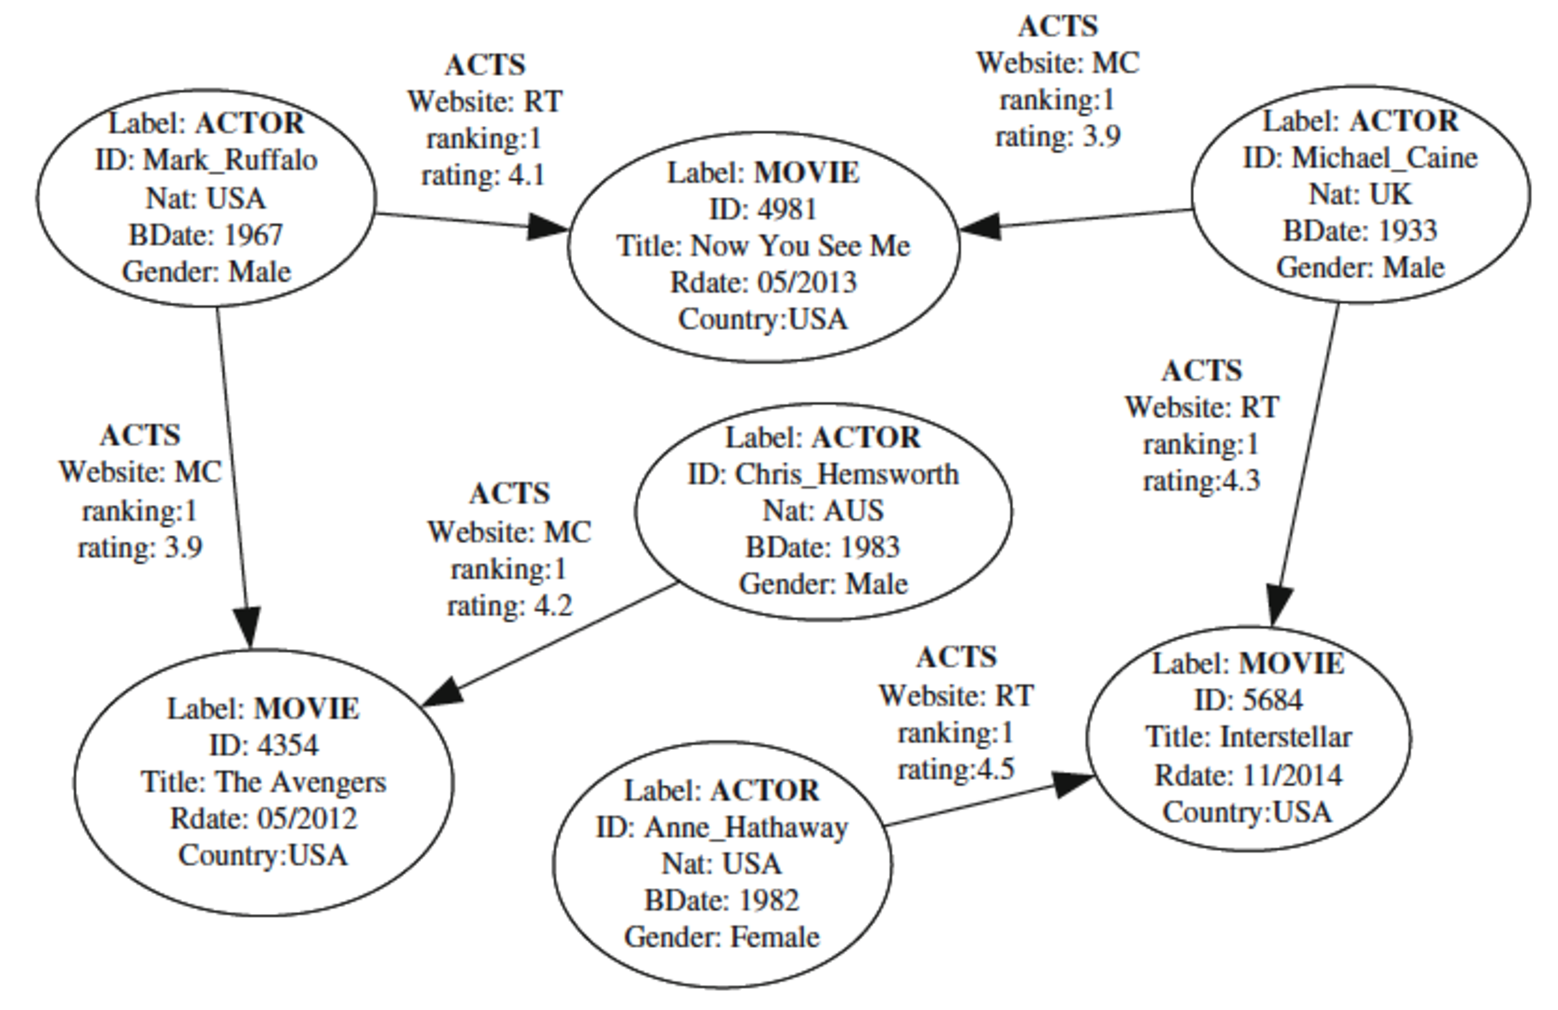
\includegraphics[width=0.8\textwidth]{../movie_graph.png}
\caption{Original movie graph \cite{ghrab2015framework}}
\label{fig:figure21}
\end{figure}

Once the dimensions are selected, a graph lattice is defined by all possible OLAP aggregations obtained by aggregating the intra-class dimensions. The inter-class measures fall back in one of the aforementioned categories (content-based,  graph-specific or graph as measure).

Figure \ref{fig:figure22} shows the aggregate graph obtained by grouping movies by their release date and actors by their birth date and gender. The graph shows the average ranking and rating of the ACTS relationship between grouped actors and movies.

\begin{figure}[ht]
\centering
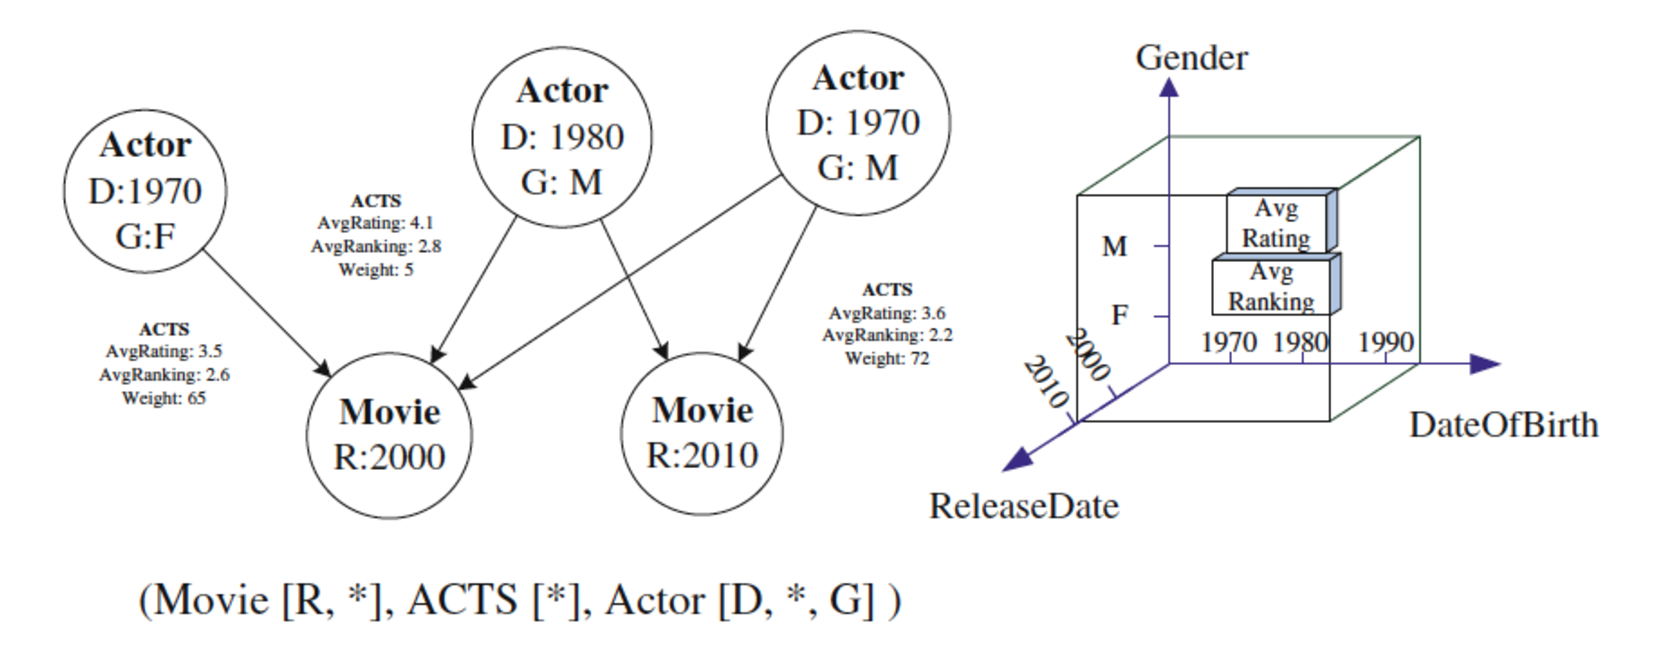
\includegraphics[width=1\textwidth]{../interclass_dimension.png}
\caption{Aggregate Graph for inter-class dimensions \cite{ghrab2015framework}}
\label{fig:figure22}
\end{figure}

This paper also proposes a technique for building OLAP cubes extracted from a graph modelled according to the analysis-oriented graph database model GRAD. This model provides advanced graph structures, integrity constraints and graph algebra. According to the authors, traditional property graphs only support OLAP analysis of inter-class dimensions, while additional capabilities brought by GRAD allows the analysis of information stored within each node.
 
The GRAD model consider heterogeneous, attributed, labelled graphs and supports complex type attributes on the nodes. This model introduces special analytical structures called hypernodes, that represent real world entities grouped by classes. Each hypernode is a subgraph formed by an entity node - which contains the label and the identifier attributes - attributes nodes - linked to the entity node and represent the non-identifier attribute - and literal nodes - which stores the effective value of its attribute node. Figure \ref{fig:figure23} shows an example of a movie graph modelled with GRAD.

\begin{figure}[ht]
\centering
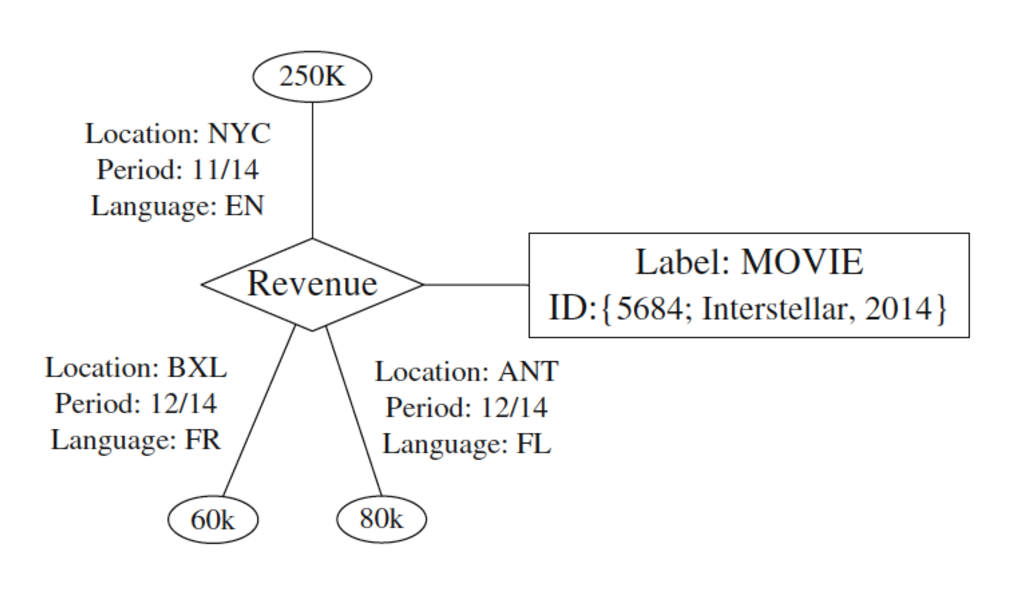
\includegraphics[width=0.5\textwidth]{../grad_model.png}
\caption{Movie graph on GRAD model \cite{ghrab2015framework}}
\label{fig:figure23}
\end{figure}

Based on this model, the paper defines Intra-class Dimensions as a subset of attributes nodes. The Intra-class Measures are identified by the attribute node label and are calculated in a similar way as the measures in property graph model. Figure \ref{fig:figure24} shows the result of applying aggregation function to the original GRAD graph in order to calculate the revenue measure, aggregating the Location according to the Country Name (CN) attribute.

\begin{figure}[ht]
\centering
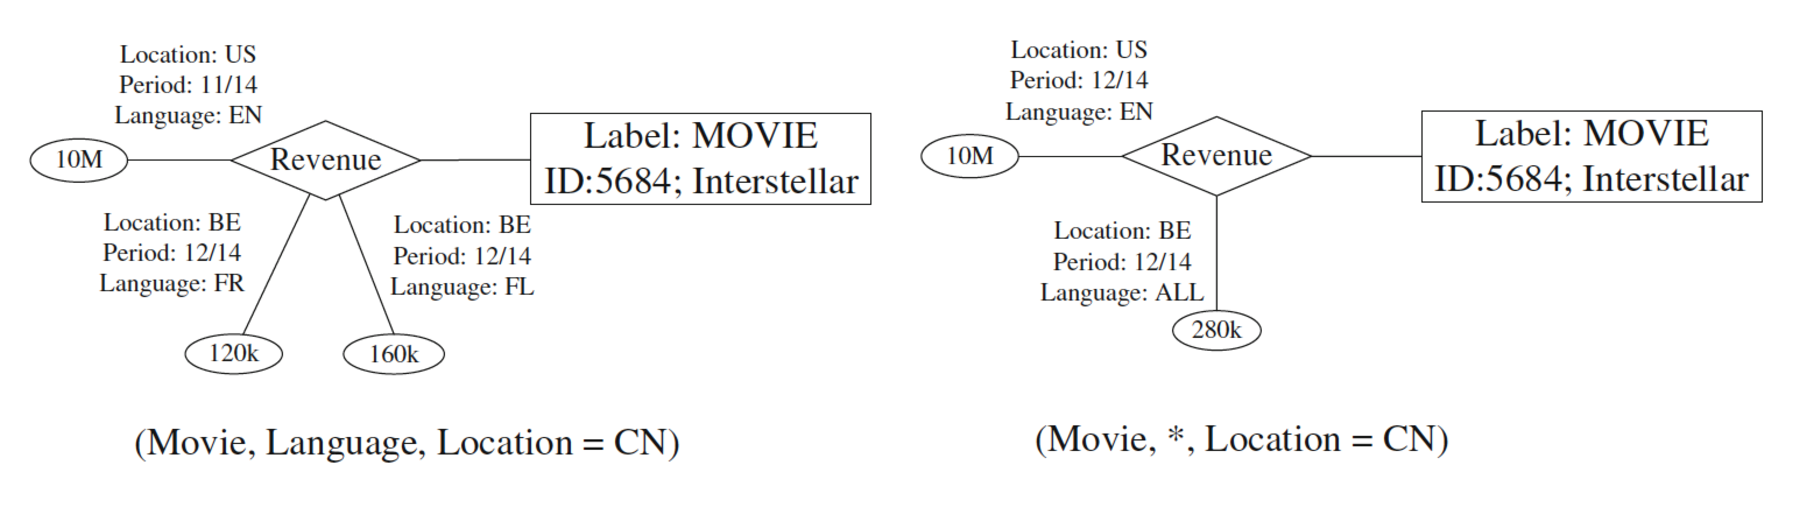
\includegraphics[width=1\textwidth]{../intraclass_dimension.png}
\caption{Aggregate Graph for intra-class dimensionl \cite{ghrab2015framework}}
\label{fig:figure24}
\end{figure}

This framework's implementation used Neo4J for the graph storage and HDFS (Hadoop Distributed File System) for distributed processing. The architecture is also composed by a middleware layer that is responsible for computing the aggregate graph and measures, using GraphX\footnote{https://spark.apache.org/graphx/} library to calculate graph-specific measures.

\section{Framework Comparison}

The first works done in OLAP analysis on graph focused on homogeneous graph datasets and defined ground concept of this area, such as aggregate graphs and graph lattice. Several operators were proposed and, in general, three types of measures were taken into consideration:
\begin{description}
\item[Informational / Content-based / Attribute-based measure] Similar to traditional OLAP measures, this information is obtained by applying an aggregate function on the node's attributes.
\item[Topological / Aggregate Graph measure] This type of measure gives information about the topology of the graph and is obtained by applying aggregate function on nodes and edges, generating a graph as a measure.
\item[Graph-based / specific measure] This type of measure is based on graph analysis theory and can be represented by a number or a subgraph.
\end{description}

One relevant characteristic of the works presented so far is the little explanation given on how the framework was indeed implemented, which made their understanding rather difficult. The Table \ref{tb:table1} shows a comparison between all the frameworks presented in this chapter, regarding the type of graph, dimensions and operations supported by each one.

\begin{table}[!ht]
\setlength\extrarowheight{2pt}
\caption{Comparison of studied frameworks}
\label{tb:table1}
\begin{tabularx}{\textwidth}{|Y|Z|Z|Z|}
\hline
\cellcolor[HTML]{C0C0C0}\textbf{Framework} & \cellcolor[HTML]{C0C0C0}\textbf{Graph} & \cellcolor[HTML]{C0C0C0}\textbf{Dimensions} & \cellcolor[HTML]{C0C0C0}\textbf{Operations}\\\hline
{\cellcolor[HTML]{EFEFEF} Graph Cube} & Homogeneous & Vertex Attributes & Cuboid and Crossboid Query\\\hline
{\cellcolor[HTML]{EFEFEF} Graph OLAP} & Homogeneous & Informational and Topological & I-OLAP and T-OLAP Operations\\\hline
{\cellcolor[HTML]{EFEFEF} HMGraph} & Heterogeneous & Informational, Topological and Entity & I-OLAP, T-OLAP, Rotate and Stretch Operations\\\hline
{\cellcolor[HTML]{EFEFEF} Pagrol} & Homogeneous & Vertex and Edge Attributes & 3 Query Category and Roll-up/Drill-down Operations \\ \hline
{\cellcolor[HTML]{EFEFEF} GRAD Graph Cubes} & Heterogeneous & Inter-class and Intra-class & - \\ \hline
\end{tabularx}
\end{table}

The work proposed here will be focused in heterogeneous graph datasets and will support the three types of measures described previously, in a similar way as presented by the work on GRAD Graph Cubes. In addition to that, this work will also explore OLAP operations on graph cubes and will perform further experiments comparing graph OLAP with traditional relational OLAP.

\section{Final Considerations}

In this chapter, we presented the main research works published related to OLAP system using Graph Databases. The majority of the works available only supported homogeneous graph, but they introduced important concepts of the area, such as graph cubes and aggregate graph. The implementations that actually gave support to heterogeneous graph, proposed different graph models in order to answer analytical queries. In the next chapter, we will specify a simple OLAP system using Graph Database without the need to define a new graph model.

\chapter{OLAP Analysis on Graph Database}
In this chapter we will propose a system capable of performing OLAP analysis and that supports heterogeneous graphs, without the need to define a new graph data model. Initially, we will contextualise the proposed system and introduce a running example that will be used to better explain the system operation. Then, the system's architecture is presented and its main components are further detailed in the following sections.

\section{Contextualisation}
In Chapter 3, we investigated some of the main works in the area of Graph OLAP. Most of them only give support to homogeneous graph \cite{Zhao2011}\cite{Chen2008}\cite{Wang2014}, while real world graph-like data contains different types of nodes and edges.The frameworks HMGraph \cite{Yin2012} and GRAD Graph Cube \cite{ghrab2015framework} support heterogeneous graph, but they propose a new multidimensional model in order to perform OLAP analysis.

The objective of the system proposed here is to support OLAP analysis on graph databases without the need to re-model operational data. This will be done by adding a layer of pre-processed aggregate graph and an analytical query processor module on top of the operational graph database.

\section{Running Example}
Consider the DBLP dataset as the running example that will be used throughout this chapter to help explaining the main concepts of the system proposed. The DBLP\footnote{http://dblp.uni-trier.de/faq/What+is+dblp.html} is an online computer science bibliography that, up until May 2016, indexes more than 3.3 million publications by more than 1.7 million authors. For this example, we will consider that the data was extracted and modelled according to the schema shown in Figure \ref{fig:figure25} and described as follows:
\begin{itemize}
\item Each publication becomes a node with label \emph{Publication} and with the attributes \emph{title}, \emph{year} and \emph{journal}.
\item Each author becomes a node with label \emph{Author} and with the attribute \emph{name}
\item Edges labeled \emph{PUBLISHED} connect Author nodes to Publication nodes, representing the relationship between an author and their published work.
\item Edges labeled \emph{COAUTHOR} connect Author nodes to other Author nodes, representing the relationship between authors that have contributed to the same published work.
\end{itemize}

\begin{figure}[ht]
\centering
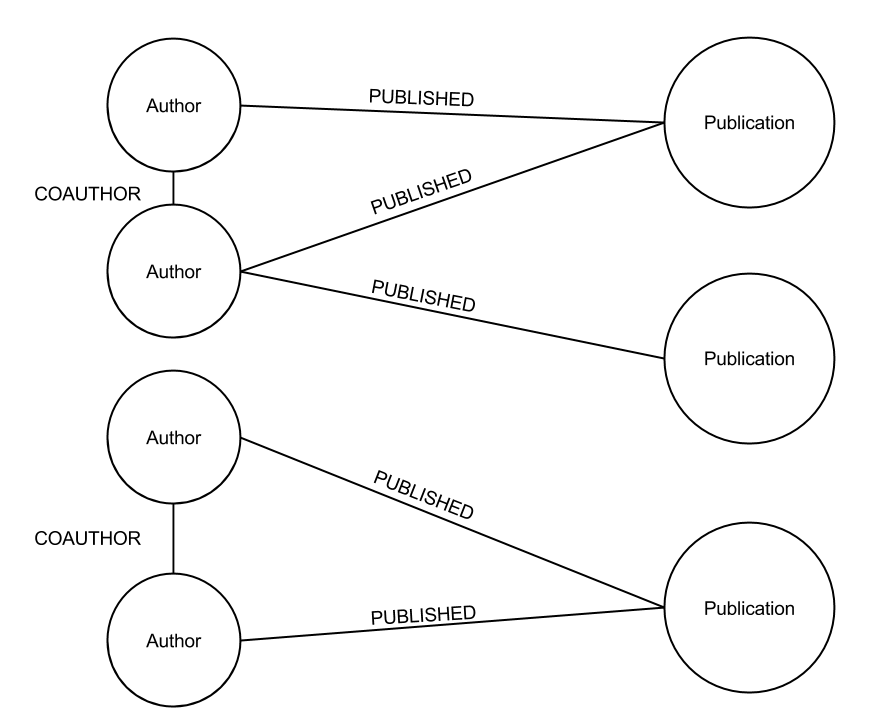
\includegraphics[width=0.7\textwidth]{../dblp_graph.png}
\caption{Schema representation of the DBLP graph data}
\label{fig:figure25}
\end{figure}

Figure \ref{fig:figure26} shows a subset of the original DBLP dataset, modelled according to the schema representation depicted in Figure \ref{fig:figure25}. The following graph will be used as our running example throughout this chapter.

\begin{figure}[ht]
\centering
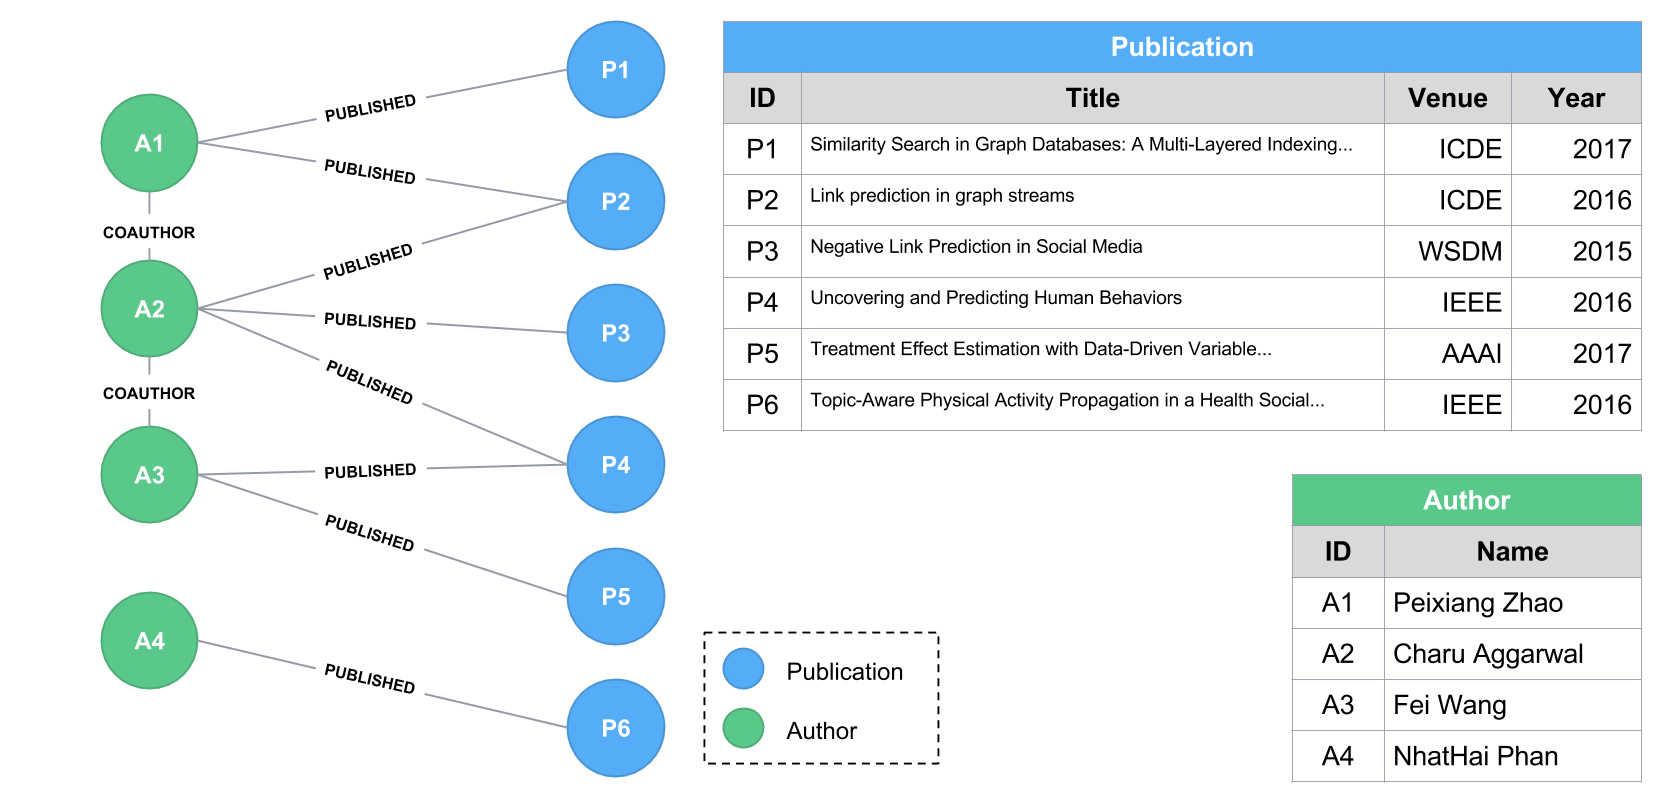
\includegraphics[width=1\textwidth]{../running_example.png}
\caption{Running Example with subset of DBLP dataset}
\label{fig:figure26}
\end{figure}

\section{Dimensions and Measures}

As discussed in Chapter 2, an OLAP system is a tool that facilitates multidimensional analysis of the data. In order to perform such kind of analysis, it is necessary to define the dimensions and measures that will be considered during the multidimensional analysis:
\begin{description}
\item[Dimension] Given a labeled property graph $G = (V, E, L_V, L_E, A_V, A_E)$, as presented in Chapter 2, a dimension is given by $d = (a, l)$, where $a \in A_V$ and $l \in L_V$. In our running example, we can define $d_1 = (journal, Publication)$ and $d_2 = (year, Publication)$, i.e. the \emph{Publication} attributes \emph{journal} and \emph{year} are dimensions $d_1$ and $d_2$ in our OLAP system, respectively.
\item[Measure] Given a labeled property graph $G = (V, E, L_V, L_E, A_V, A_E)$, a measure $m$ is a calculation computed over the graph $G$ using a function $F$ ($m=F(G)$), that can return the type of measures defined by  \cite{ghrab2015framework}:
\begin{description}
\item[Content-based measure] For this kind of measure is calculated based on the nodes and edges attributes and the function $F \in \{SUM, COUNT, AVG, \dots\}$ used in the calculation are similar to the ones used in an OLAP system. In our running example, the total number of authors that published a work in 2007 is a content-based measure that is calculated using the function $COUNT$, which will count the number of \emph{Author} nodes that have a relationship \emph{PUBLISHED} to \emph{Publication} nodes that have attribute \emph{year} equals to 2007.
\item[Graph-specific measure] This type of measure is calculated by applying a network analysis algorithm over the graph, i.e. a network analysis algorithm is used as the function $F$. In our running example, the list of authors that most contributed with other authors is a graph-specific measure that is computed by applying the degree centrality measure to the \emph{Author} nodes of the graph.
\item[Graph as measure] This kind of measure is given by different aggregation levels of a graph and the function $F$ that calculates this measure is the aggregate function that will generate the aggregate graph. In our running example, the network of authors and  publications aggregated according to the journal the work was published in is a graph that represents a measure.
\end{description}
\end{description}

\section{Architecture}

The Graph OLAP system proposed in this work attempts to provide an efficient way to answer analytical queries without having to propose a new graph data model, which would imply changing the original data source model. The Figure \ref{fig:figure27} depicts the architecture of the system, illustrating its main components: Graph Aggregators, Aggregated Graphs and Analytical Query Processor.

The Graph Aggregators are modules that are responsible for processing the original data and generate Aggregate Graphs, which are stored in Graph Databases. The Analytical Query Processor is in charge of processing the incoming query and determine whether it should be answered by processing the original or the aggregate date, based on the type of measure being analysed.

\begin{figure}[ht]
\centering
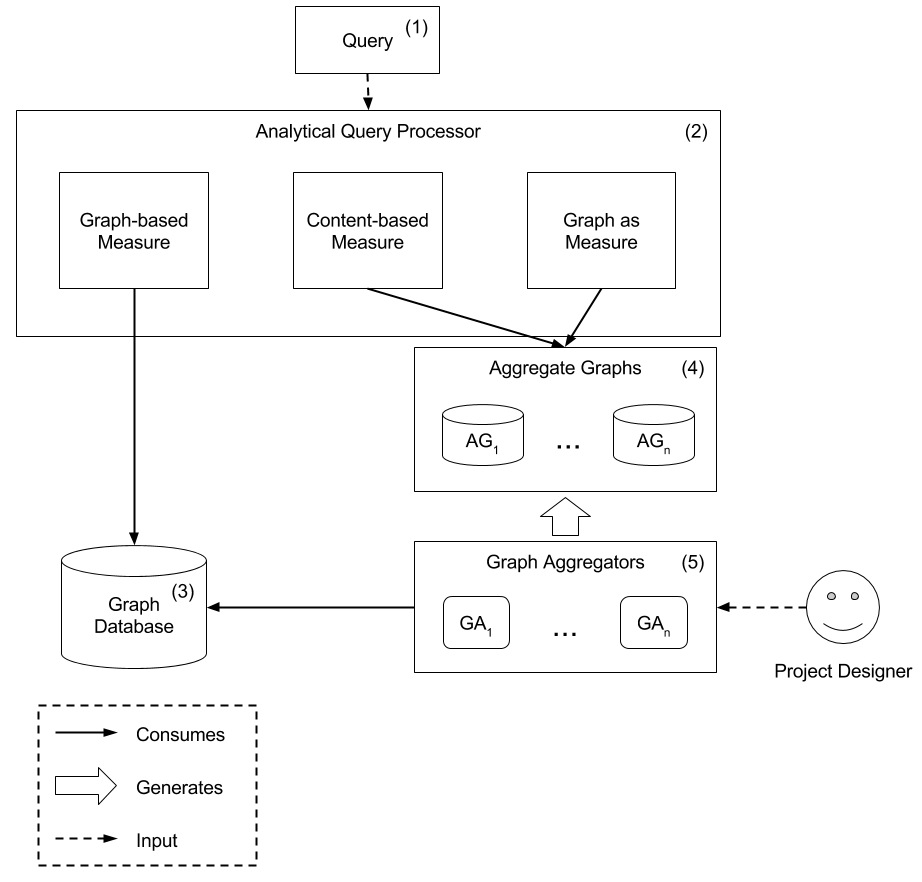
\includegraphics[width=0.8\textwidth]{../Architecture.png}
\caption{OLAP Analysis over Graph Databases Architecture}
\label{fig:figure27}
\end{figure}

The system's input is an analytical query submitted by the user, that will be processed by the Analytical Query Processor (AQP). According to the type of measure expected by the user, the AQP will determine which specific processor will handle the query: graph-based, content-based or graph measures processors. If the user asks for a graph-based measure, the AQP will consume the original data stored in the graph database to calculate the measure. On the other hand, if the user requires a content-based or a graph as measure, the AQP will calculate the measure based on the data from Aggregate Graphs, which are also stored in graph databases.

The Aggregate Graphs are generated by the Graph Aggregators (GAs), which are defined during the design process of the system by the project designer. The project designer is responsible to define what are the dimensions considered in the OLAP system and, therefore, create the GAs that will generate all possible aggregate graphs for the dimensions. More details on Aggregate Graphs and Graph Aggregators are given in the following sections.

The data source considered for this system is a Graph Database that follows the labeled property graph model and supports heterogeneous graphs. This means that nodes can have one or more labels indicating different types of entities. Nodes and relationships can have properties. We assume that the data stored in the GDB is integrated, i.e. the data in the repository is consistent, well-formatted and normalised.

\section{Aggregate Graph}
Given a graph $G = (V, E, L_V, L_E, A_V, A_E)$ and a set of dimensions $D = \{d_1, \dots, d_n\}$, where $d_i \in A_V \cup A_E$, an aggregate graph is generated by applying an aggregate function $F$ to one or more dimensions. The result is a new graph $G_A = (V_A, E_A, L_{VA}, L_{EA}, A_{VA}, A_{EA})$, where:
\begin{itemize}
\item $VA = \{v^A_1, \dots, v^A_n\}$ is a set of aggregate vertices, where each vertex $v^A_i$ either (i) corresponds to the result of applying the function $F$ to a set of vertices $V' \subseteq V$ that is associated with an attribute vector $[a_1, \dots, a_k]$ containing one or more dimensions in $D$ or (ii) corresponds to a vertex in $V$.
\item $E_A \subseteq V_A \times V_A$ is a set of aggregate edges, where each edge $e^A_i$ either (i) corresponds to the result of collapsing a set of edges $E' \subseteq E$ that connects one or more vertices in $V$ that were aggregated in $V_A$ or (ii) corresponds to an edge in $E$.
\item $L_{VA}$ is a set of aggregate vertex labels and $L_{EA}$ is a set of aggregate edge labels
\item $A_{VA} = \{a_1, \dots, a_n\}$ is the set of attributes for the aggregate vertices, where $a_i = (k_i, m_i)$ is a key-value pair. Each aggregate vertex $v_i \in V_A$ is associated with an attribute vector. $A_{EA} = \{b_1, \dots, b_n\}$ is the set of aggregate edge attributes defined in the same way as aggregate vertices attributes.
\end{itemize}

Consider the graph depicted in Figure \ref{fig:figure26} of our running example. Figure \ref{fig:figure28} shows the aggregate graph $G_A$ obtained by applying the aggregate function COUNT to the dimension set $D = \{d\}$, where $d = (year, Publication)$. Notice that the resulting aggregate graph ends up with the same \emph{Author} nodes as the original graph, since these vertices do not have attributes contained in the dimension set $D$. The \emph{Publication} nodes were aggregated according to their \emph{year} attribute, resulting in three nodes representing the works published in 2017, 2016 and 2015. The aggregate vertices also store the measure calculated using the function COUNT. The edges with the label PUBLISHED were collapsed, representing the connection between each author and the group of works published in a specific year. The collapsed edges also store the measure obtained by the use of COUNT function.

\begin{figure}[ht]
\centering
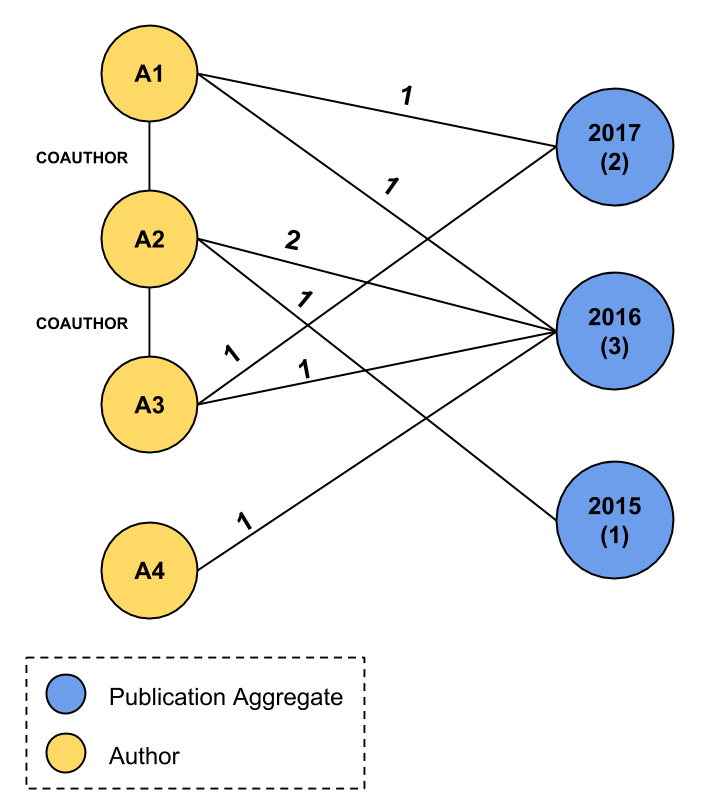
\includegraphics[width=0.6\textwidth]{../aggregate_graph_running_example.png}
\caption{Aggregate Graph obtained from running example graph}
\label{fig:figure28}
\end{figure}

\section{Graph Aggregators}

The Graph Aggregators (GAs) are modules responsible for generating the aggregate graph that will be used to answer the analytical query submitted by the user. During the design process for the system, the Project Designer is responsible for building the GAs based on the dimensions and measures the system should be able to analyse. Each GA will receive as input the original graph G stored in the Graph Database, the set of dimensions to be aggregated D, the aggregate function F and should provide as output an aggregate graph as defined in the previous section. Algorithm \ref{alg:algorithm1} describes the process performed by a GA in order to generate an aggregate graph.

\begin{algorithm}
 \caption{Graph Aggregator Process}\label{alg:algorithm1}
  \begin{algorithmic}[1]
    \Function{$generateAggGraph$}{$G, F, D$}
      \State{$aggVertices \gets []$} \label{alg:line2}
      \State{$aggEdges \gets []$} \label{alg:line3}
      \For{$ node \textrm{ in } G.vertices$}  \label{alg:line4}
        \If {$ node.label  \textrm{ in } D $}  \label{alg:line5}
          \State{$dimValue \gets getDimValue(node, D)$}
           \If {$ dimValue  \textrm{ in } aggVertices $}  \label{alg:line7}
             \State{$aggregateVertices(dimValue, node, F)$}  \label{alg:line8}
             \State{$aggregateEdges(dimValue, node, F)$}  \label{alg:line9}
           \Else
              \State{$aggVertices.add(dimValue, node)$}  \label{alg:line11}
              \State{$aggregateEdges(dimValue, node, F)$}  \label{alg:line12}
           \EndIf
       \Else
          \State{$aggVertices.add(node)$}  \label{alg:line15}
        \EndIf
      \EndFor
      \State{$aggGraph \gets (aggVertices, aggEdges)$}  \label{alg:line18}
      \State \Return{$aggGraph$}  \label{alg:line19}
    \EndFunction
  \end{algorithmic}
\end{algorithm}

The GA algorithm starts by creating an empty set of aggregate vertices and edges (lines \ref{alg:line2} and \ref{alg:line3}) that will compose the final aggregate graph that will be returned. Then, the GA will iterate over all the vertices (nodes) of the original graph G (line \ref{alg:line4}), checking for each node if it has the same label as the dimension being aggregated (line \ref{alg:line5}). If the node has the same label, the algorithm checks if already exists an aggregate node for the dimension value of the node (line \ref{alg:line7}). If the aggregate node exists, we collapse the value of the node to the value of the aggregate node using the function F and updating the aggregate node value (line \ref{alg:line8}). We also aggregate the edges that are connected to the node accordingly (line \ref{alg:line9}). If the aggregate node does not exist, we add a new aggregate node with the initial value equals to node's dimension value and aggregate its edges accordingly (lines \ref{alg:line11} and \ref{alg:line12}). If the node does not have the same label as the dimension being aggregated, we only add the node as it is to the aggregate vertices set (line \ref{alg:line15}). Finally, we setup the aggregate graph and return it (lines \ref{alg:line18} and \ref{alg:line19}).

Once the aggregate graph is generated, it will be stored in a graph database and it will be accessed by the Analytical Query Processor.

\section{Analytical Query Processor}

The Analytical Query Processor (AQP) is responsible for processing the query submitted by the user. This component contains three modules that will process the query differently based on the type of measure requested by the user:
\begin{description}
\item[Graph-based measure] To calculate this measure, the AQP consumes the data from the original graph database and uses any existing library to perform network analysis on the data. 

In our running example, we could submit a query asking for the \emph{Author} node with highest centrality degree. The AQP calculates the centrality degree for each node in the original graph using an external library. Then, it should return the node with id \textbf{A2}, since it is the Author node with the highest number of connections with other nodes.

\item[Content-based measure] To calculate this measure, the AQP consumes the data from an aggregate graph and uses the aggregate function to give the resulting measure, which can be a single value, a list or a table of values. This module's response is similar to the response given by traditional OLAP systems.

From our running example, we can ask for the count of publications by year. In this case AQP consumes the data from the aggregate graph illustrated in Figure \ref{fig:figure28} and it would list the nodes with \emph{Publication Aggregate} label, which already contains the count measure as attribute.

\item[Graph as measure] For this type of measure, the AQP also consumes data from an aggregate graph, but in this case, the measure is the aggregated graph itself. Therefore, this module does not need to perform other calculations.

For instance, the aggregate graph shown in Figure \ref{fig:figure28} can be considered a measure if the user requests a topological view of the original data grouping the publications by year
\end{description}

\section{Final Considerations}
In this chapter, we showed the main components of the proposed system and what is the general flow to answer an analytical query. We also specified in details how each one of the components works and what are their roles in the data analysis process. In the next chapter, we will report how the proposed system was implemented and show some experiments and the results obtained.

\chapter{Implementation and Experiments}

In this chapter, we will show how the system specified in the Chapter 4 was implemented and what were the technologies used. We will also describe the experiments made and analyse the results obtained in comparison to existing solutions. Finally, we will discuss the difficulties found in the implementation and experimentation process.

\section{Used Technologies}
The Graph Aggregator (GA) algorithm were implemented using Python programming language, in version 2.7. The original data and the aggregate graphs were stored in a Neo4J database. In order to the GA connect to the Neo4J database, it was necessary to use the Python library Py2Neo, in version 3.1.2. The Analytical Query Processor uses the compiler built in Neo4J and the query accepted as input to the system is written using Cypher query language.

\subsection{Neo4J}
As mentioned in Chapter 2, Neo4J is the most popular graph database in the industry according to DB Engines website. In comparison with other DBs from the same category, Neo4J has a good performance considering time to process a query and the amount of memory consumed by the database.

The queries submitted to Neo4J are written in Cypher \cite{Neo4jCypher}, which is a declarative query language inspired by SQL and that describes graph patterns using ASCII characters. Figure \ref{fig:figure29} shows an example of how cypher represents a relationship in the query syntax. This language also allows to create, update and delete nodes and relationships.

\begin{figure}[ht]
\centering
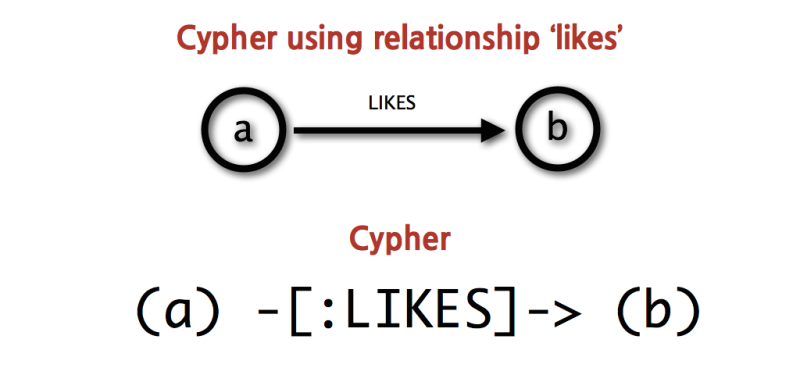
\includegraphics[width=0.6\textwidth]{../cypher_pattern_simple.png}
\caption{Cypher syntax representation of a relationship in the graph \cite{Neo4jCypher}}
\label{fig:figure29}
\end{figure}

Neo4J query language also includes a series of clauses and expressions similar to SQL, such as  $WHERE$, $ORDER BY$, $LIMIT$, $AND$, among others. The Cypher query shown in Figure \ref{fig:figure30} is an example of the general syntax of the language and it shows how it is possible to restrict the results by a certain threshold using the clause $WHERE$. The mentioned query will return a subgraph containing the nodes with labels Label1 and Label2 that have a relationship of type \emph{TYPE} with a property value above a certain threshold.

\begin{figure}[ht]
\centering
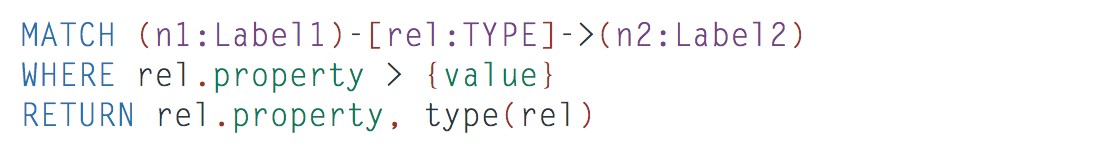
\includegraphics[width=0.8\textwidth]{../cypher_general_syntax.png}
\caption{Example of Cypher Query syntax \cite{Neo4jCypher}}
\label{fig:figure30}
\end{figure}

The data stored in a Neo4J database can be accessed using a Java API or a REST API by default. In order to facilitate the access to the data using a Python application we used an external library called Py2Neo, which wraps REST API requests to perform Cypher commands on the database. In this way, it was possible to implements the algorithm for the Graph Aggregators, where it consumes the original data, generate an aggregate graph and stores it in another instance of a Neo4J database.

Another interesting feature in Neo4J is its web-based user interface. This interface provides a direct way to submit Cypher queries to the database and a visualisation of the results. Figure \ref{fig:figure31} is a screenshot if the interface, showing the result of a simple query submitted in the text area at the top of the screen. The submitted query returns a subgraph showing the relationship between the Author Felix Naumann with all his publications present in the database. The interface shows each node as a circle and relationship as an arrow, it also shows the properties and labels of nodes and relationships when they are clicked. The experiments shown in this chapter will be displayed using the graphic interface provided by Neo4J.

\begin{figure}[ht]
\centering
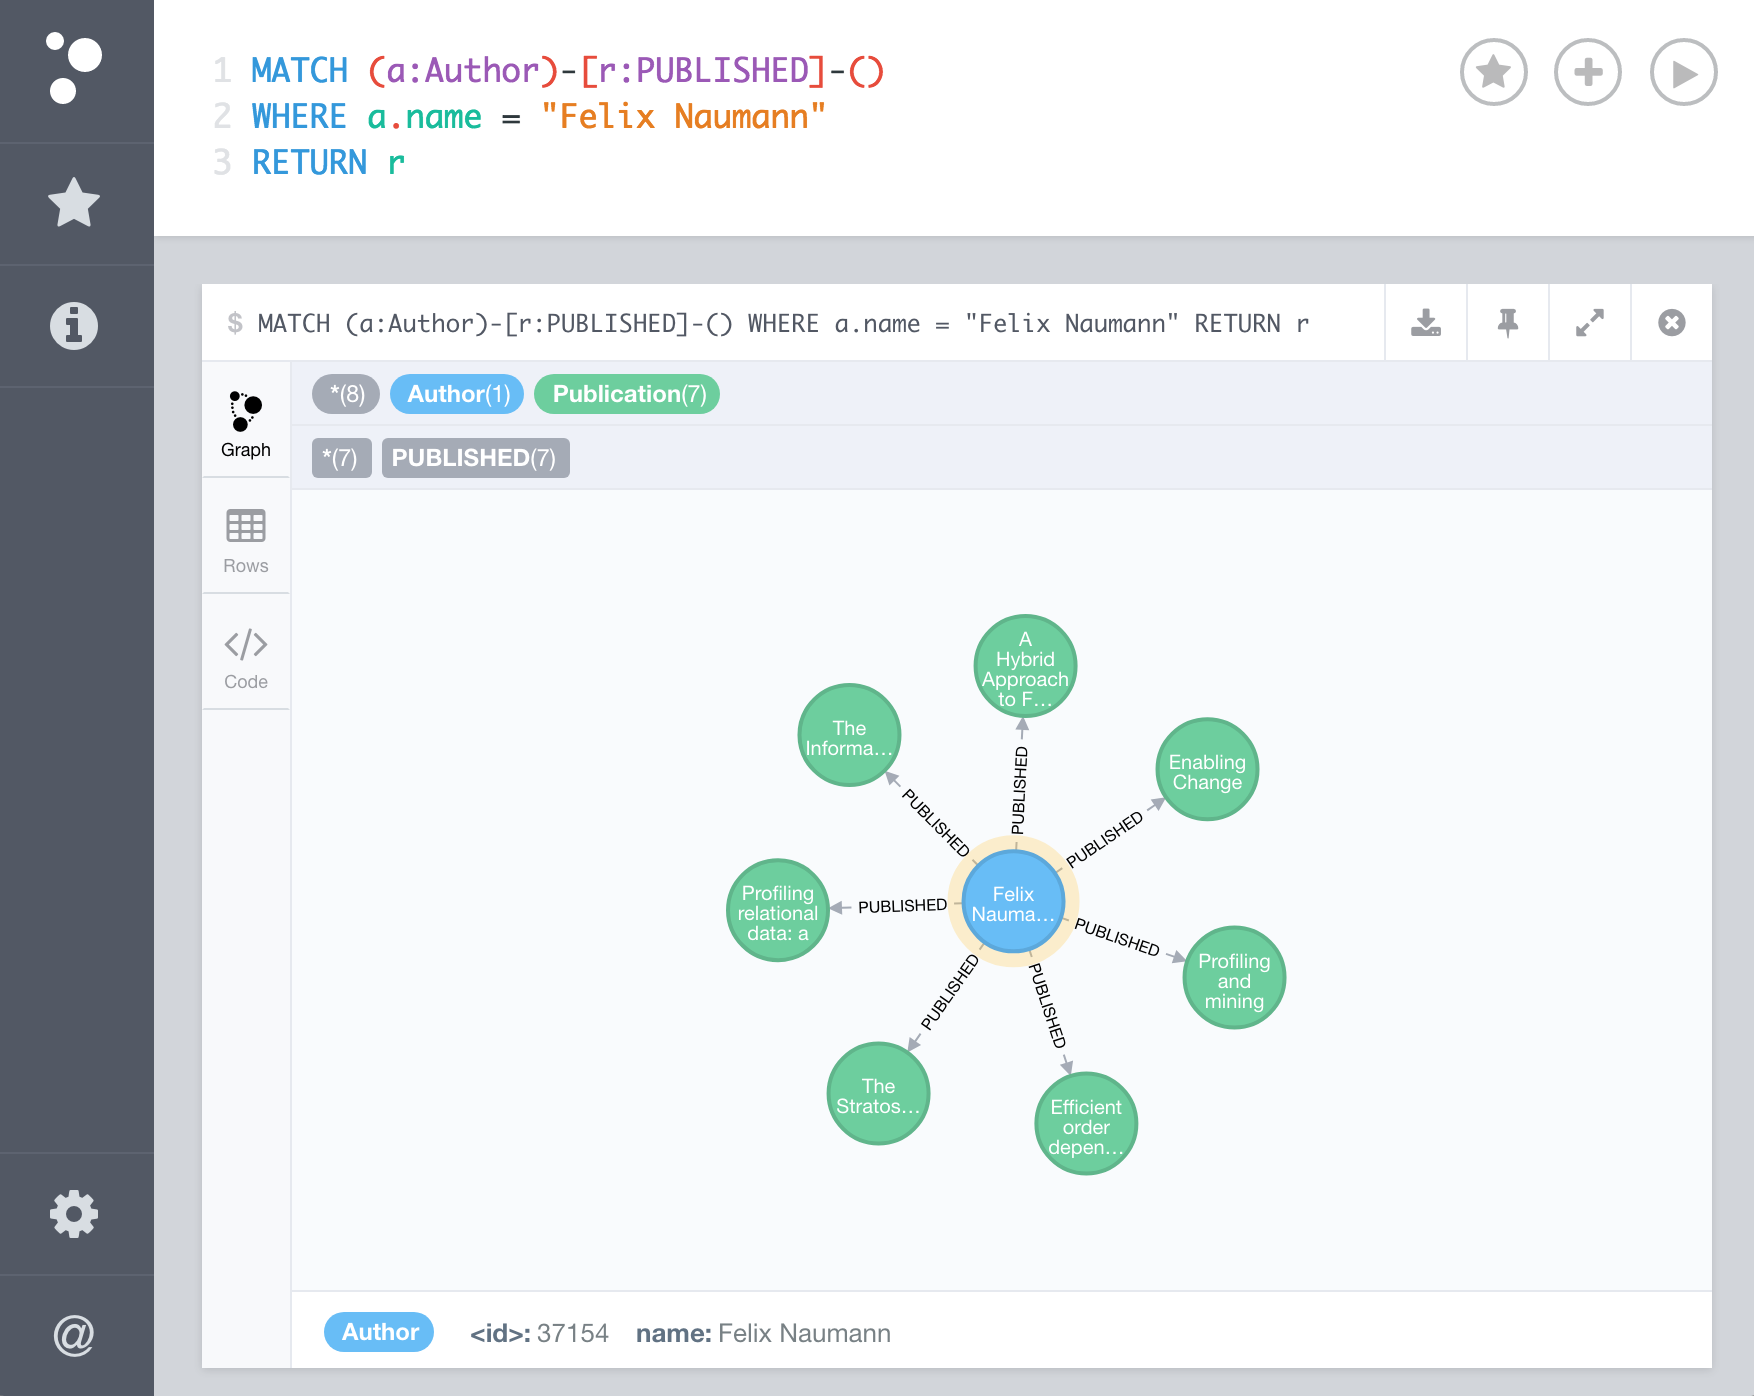
\includegraphics[width=1\textwidth]{../neo4j_user_interface.png}
\caption{Neo4J User Interface}
\label{fig:figure31}
\end{figure}

\section{Data set}

The data set used for the experiments was the Database System and Logic Programming (DBLP) computer science bibliography, available in [ref], which contains more than 3.8 million publications published by more than 1.7 million authors. The dataset can be downloaded as a XML file accompanied by a DTD file that describes the schema of the data. The code in \ref{lst:listing1} is a snippet of the DBLP XML file showing how a publications is structured in the document.

\lstset{breaklines=true,
	caption={DBLP XML File Snippet},
	label={lst:listing1},
	captionpos=b, 
	frame=single,
	morekeywords={article, author, title, pages, year, volume, journal, number, ee, url, mdate, key}}

\begin{lstlisting}
<article mdate="2017-01-03" key="journals/jacm/GanorKR16">
  <author>Anat Ganor</author>
  <author>Gillat Kol</author>
  <author>Ran Raz</author>
  <title>Exponential Separation of Information and Communication for Boolean Functions.</title>
  <pages>46:1-46:31</pages>
  <year>2016</year>
  <volume>63</volume>
  <journal>J. ACM</journal>
  <number>5</number>
  <ee>http://dl.acm.org/citation.cfm?id=2907939</ee>
  <url>db/journals/jacm/jacm63.html#GanorKR16</url>
</article>
\end{lstlisting}

The snippet shown in \ref{lst:listing1} refers to an article published in J. ACM journal and it contains information about the article's authors, title, pages in journal, year of publication and other informations about the journal's volume, number and electronic edition location. Each publication also has a unique key and the date of the last modification as attributes and an element with the url of the publication in the DBLP website. Besides journal articles, the DBLP dataset also contains books, thesis, conferences and workshops papers, among others.

Once the XML file was downloaded, all the data was parsed and stored into a SQLite database. In order to have a more controlled environment for the experiments, we selected a subset of the original data, considering only papers and articles published in the following conferences and journals since 2014:

\begin{itemize}
\item SIGMOD International Conference on Management of Data (SIGMOD)
\item Brazilian Symposium on Databases (SBBD)
\item International Conference on Very Large Databases (VLDB)
\item IEEE International Conference on Data Engineering (ICDE)
\item World Wide Web: Internet and Web Information Systems (WWW)
\end{itemize}

The selected subset of publications was imported to a Neo4J instance, following the schema depicted in Figure \ref{fig:figure32}. Each publication became a node in the graph database, with three attributes: (i) the title; (ii) the year of publication and (iii) the acronym of the journal or conference. The authors of each publication also became a node, uniquely identified by the name of the author, and they are connected with the publications node by a relationship of type PUBLISHED. Authors that have contributed in the same publication are also connected by a relationship of type CO\_AUTHORSHIP.

\begin{figure}[ht]
\centering
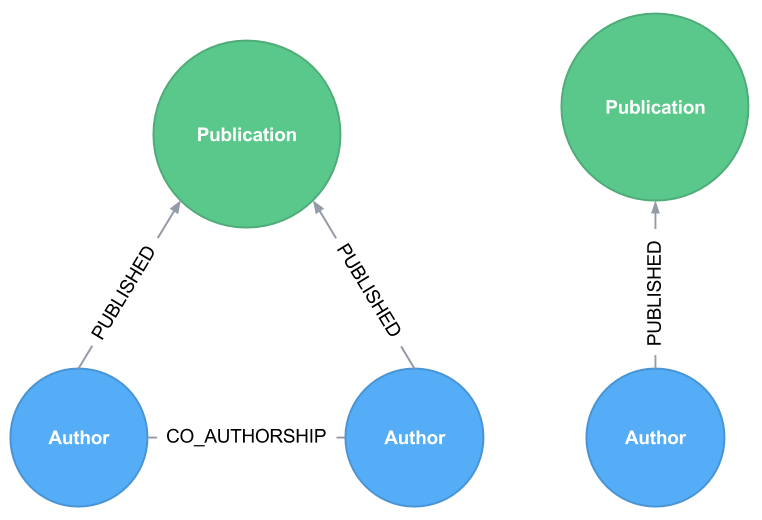
\includegraphics[width=0.6\textwidth]{../dblp_schema.png}
\caption{DBLP dataset schema in graph database}
\label{fig:figure32}
\end{figure}

By the end of the DBLP subset loading process to Neo4J, we had 887 Publication nodes, 2.398 Author nodes, 6.754 PUBLISHED relationships and 25.572 CO\_AUTHORSHIP relationships.

\section{Experiments and Results}
With the Neo4J database loaded with DBLP data, we executed the Graph Aggregator (GA) algorithm passing as parameters the dimensions year and journal/conference of a Publication node and the COUNT aggregate function. Figure \ref{fig:figure33} shows a subgraph of the aggregate graph generated by the GA, with one aggregate node representing all the publications on ICDE 2016 and some of the authors that published on that conference, that year. From the measure attribute of the aggregate node, we know that ICDE had 60 publications in 2016.

\begin{figure}[ht]
\centering
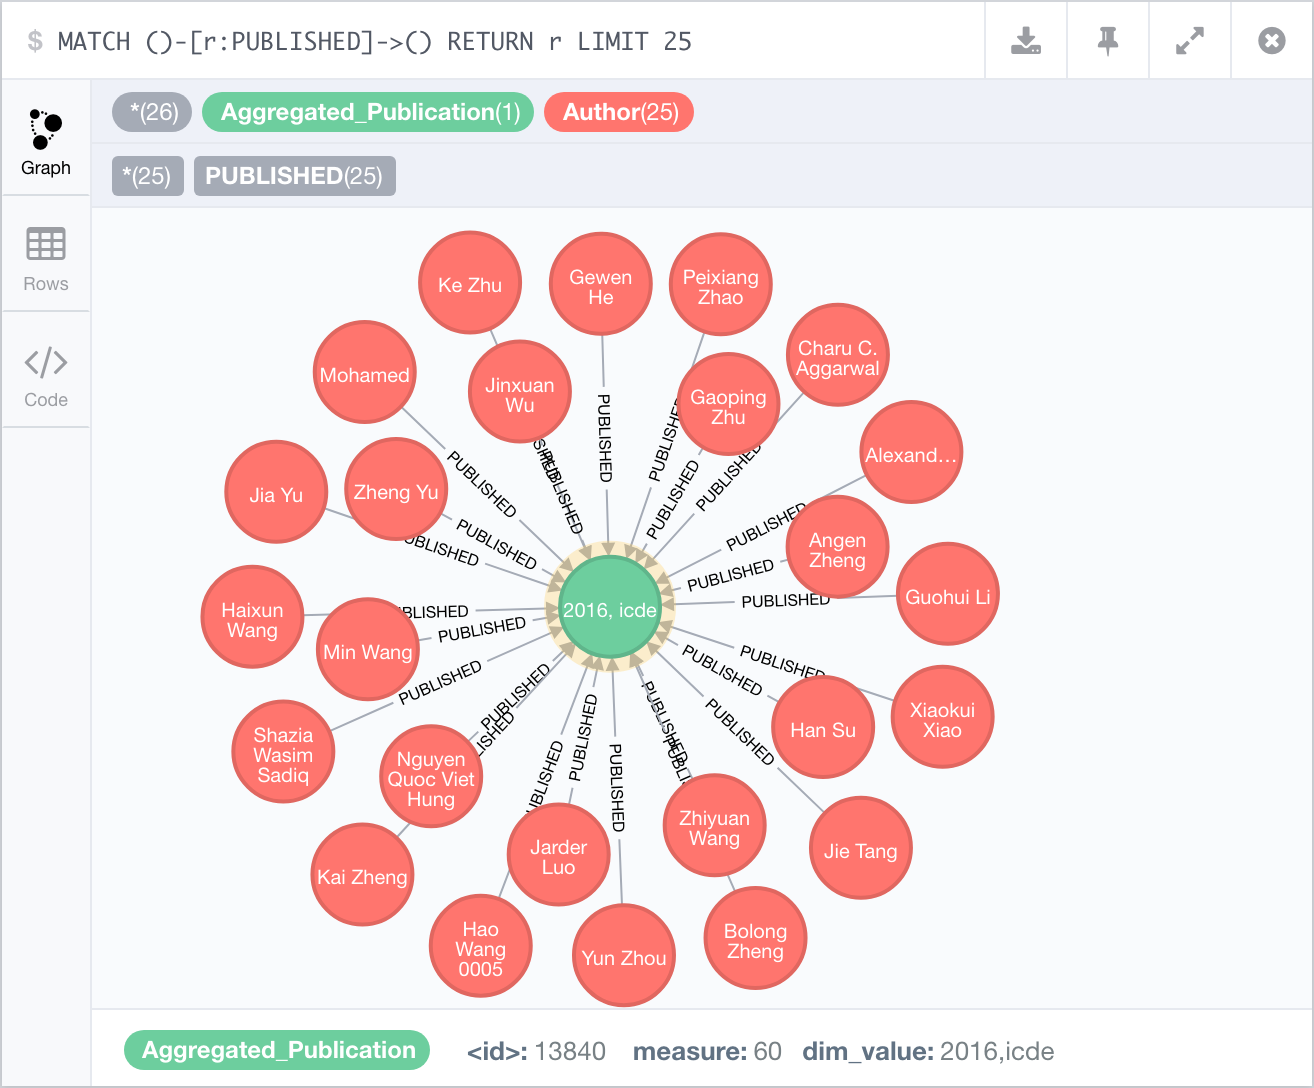
\includegraphics[width=1\textwidth]{../aggregate_graph_subgraph.png}
\caption{Subgraph from the Aggregate Graph generated by the GA}
\label{fig:figure33}
\end{figure}

Once we generated the aggregate graph, we were able to perform an experiment to evaluate the effectiveness of the proposed system. For that, we submitted queries to calculate the three type of measures supported: content-based, graph-specific and graph as measure.

\subsection{Content-based Measure}
For this type of measure, we submitted a query asking for the amount of publications by journal / conference in the year of 2016. This query was submitted to the aggregate graph generated by the GA and it returns all the nodes with the label Aggregate\_Publication where the dimension year has the value 2016. The result is then ordered by the number of publications measure.

Figure \ref{fig:figure34} depicts the result of the query, listing the conferences and journals ordered by the amount of publications in the year of 2016. The conference SIGMOD appears at the top of the list with 61 publications for that year. In comparison to a traditional relational OLAP system, this query is corresponding to a slice operation, in which we slice a part of the journal dimension based on the value of the dimension year.

\begin{figure}[ht]
\centering
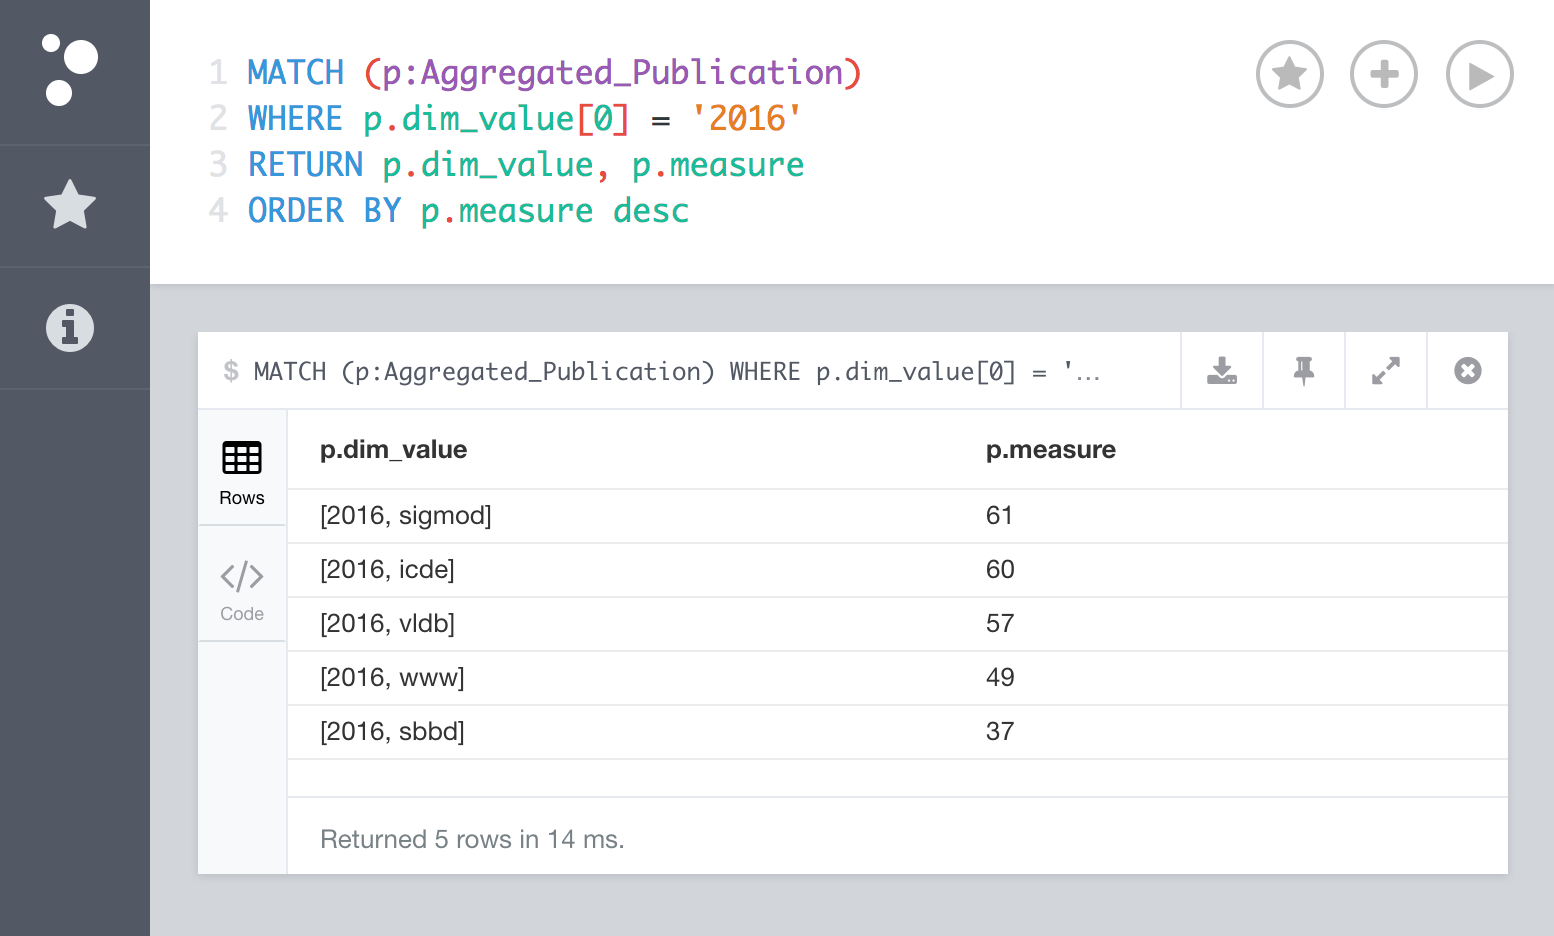
\includegraphics[width=1\textwidth]{../exp_content_measure.png}
\caption{Result of experiment with a content-based measure query}
\label{fig:figure34}
\end{figure}

\subsection{Graph-specific Measure}
In order to test this type of measure, we submitted two centrality measures queries to the original dataset in the graph database. The first measure calculated was the degree centrality of each Author node considering the CO\_AUTHORSHIP relationship. As mentioned in Chapter 2, the degree centrality is given by the count of adjacent node, i.e. the count of CO\_AUTHORSHIP relationship an Author node has.

Figure \ref{fig:figure35} shows the result of the centrality measure query, listing the 10 authors with the highest degree centrality in the original network. For our dataset, Michael J. Franklin is the author with the highest number of adjacent Author nodes, which means that he is one of the focal points in the network.

\begin{figure}[ht]
\centering
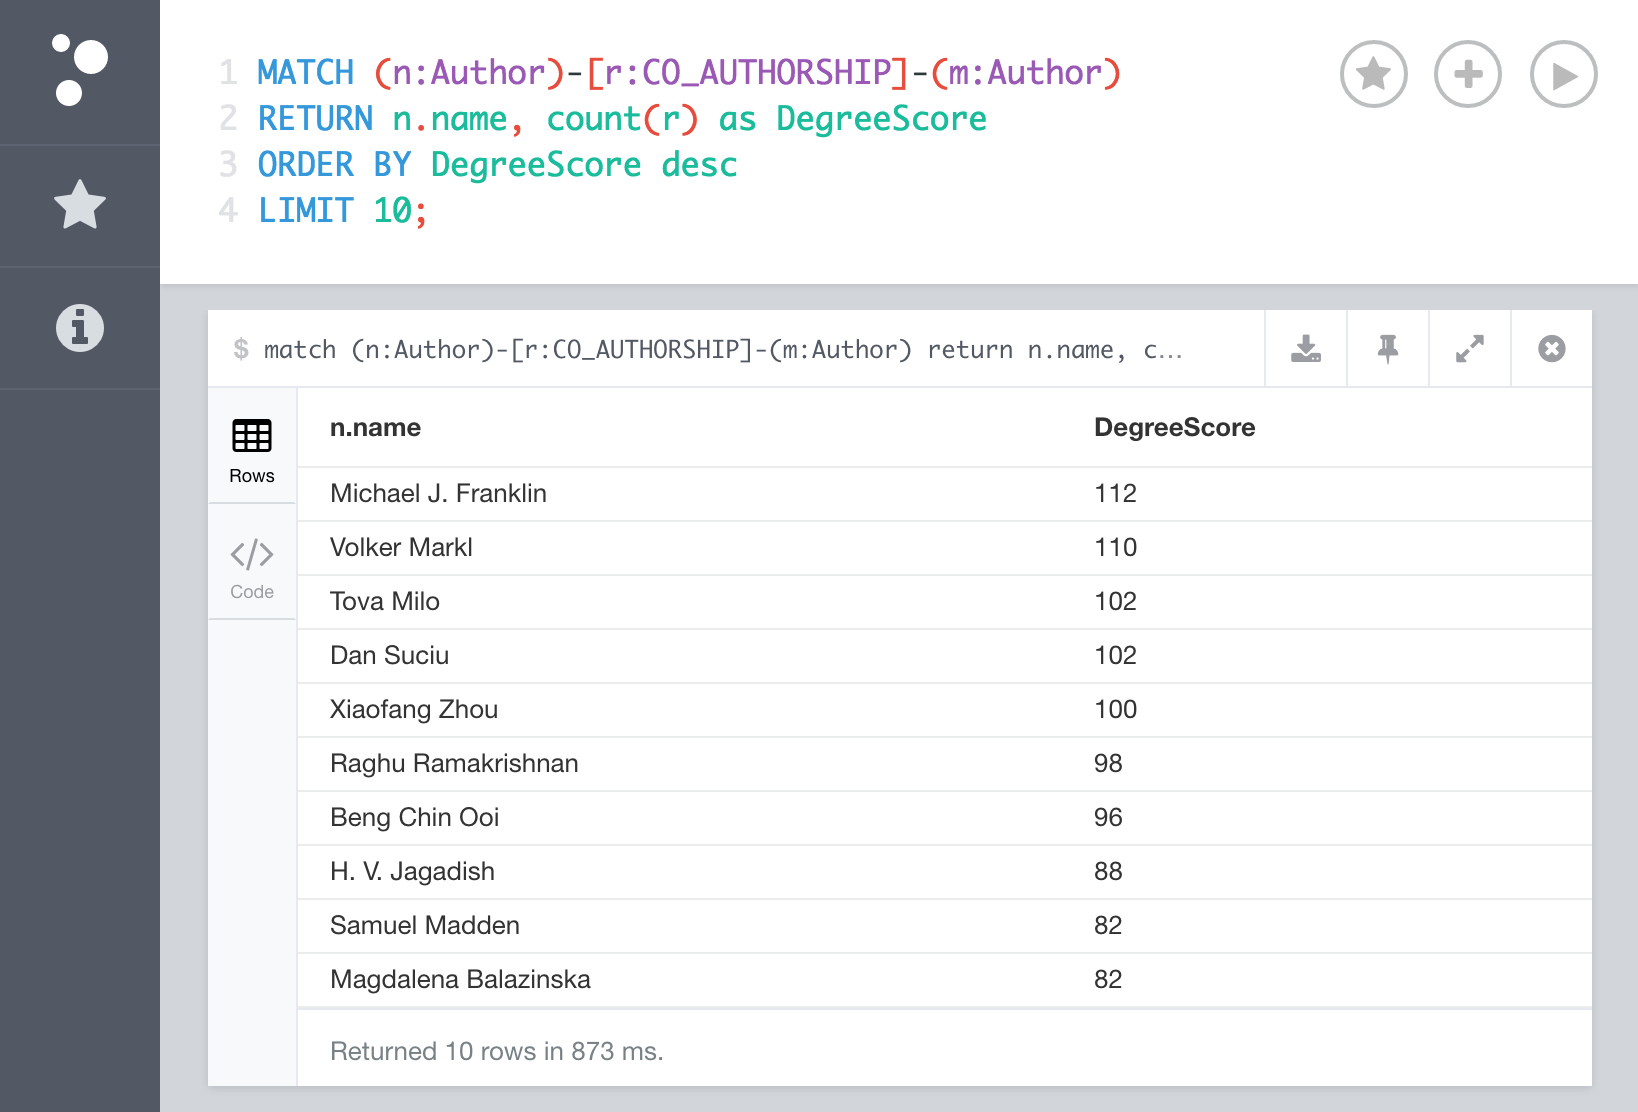
\includegraphics[width=1\textwidth]{../exp_degree_centrality.png}
\caption{Result of experiment with the degree centrality measure for Authors}
\label{fig:figure35}
\end{figure}

The second measure calculated was the betweenness centrality of the authors. This centrality measure is given by the frequency in which an author node appears in the shortest path of any other two author nodes in the graph. In Cypher, there is a built-in function to retrieve all shortest path between two nodes called $allShortestPaths$. Since getting all the shortest path between the combination of any 2 nodes in the graph is such a complex computation, we considered the paths with maximum 3 degrees of separation and we avoided inverse relationships by comparing the id of the nodes. Finally, we returned the 10 authors that most appeared in the list of the shortest paths.

Figure \ref{fig:figure36} shows the result of author's betweenness centrality calculation. Reaffirming his importance in the co-authorship network, Michael J. Franklin appears again in the first position of the list, meaning that he is an important point of transmitting information between authors. One interesting result is related to the second place for both experiments: the second author with the highest degree centrality is not the same as the second author with the highest betweenness centrality. This means that, even so Volker Marki co-authored publications with more authors than Beng Chin Ooi, the latter is a more important channel of information between two other authors in the network.

\begin{figure}[ht]
\centering
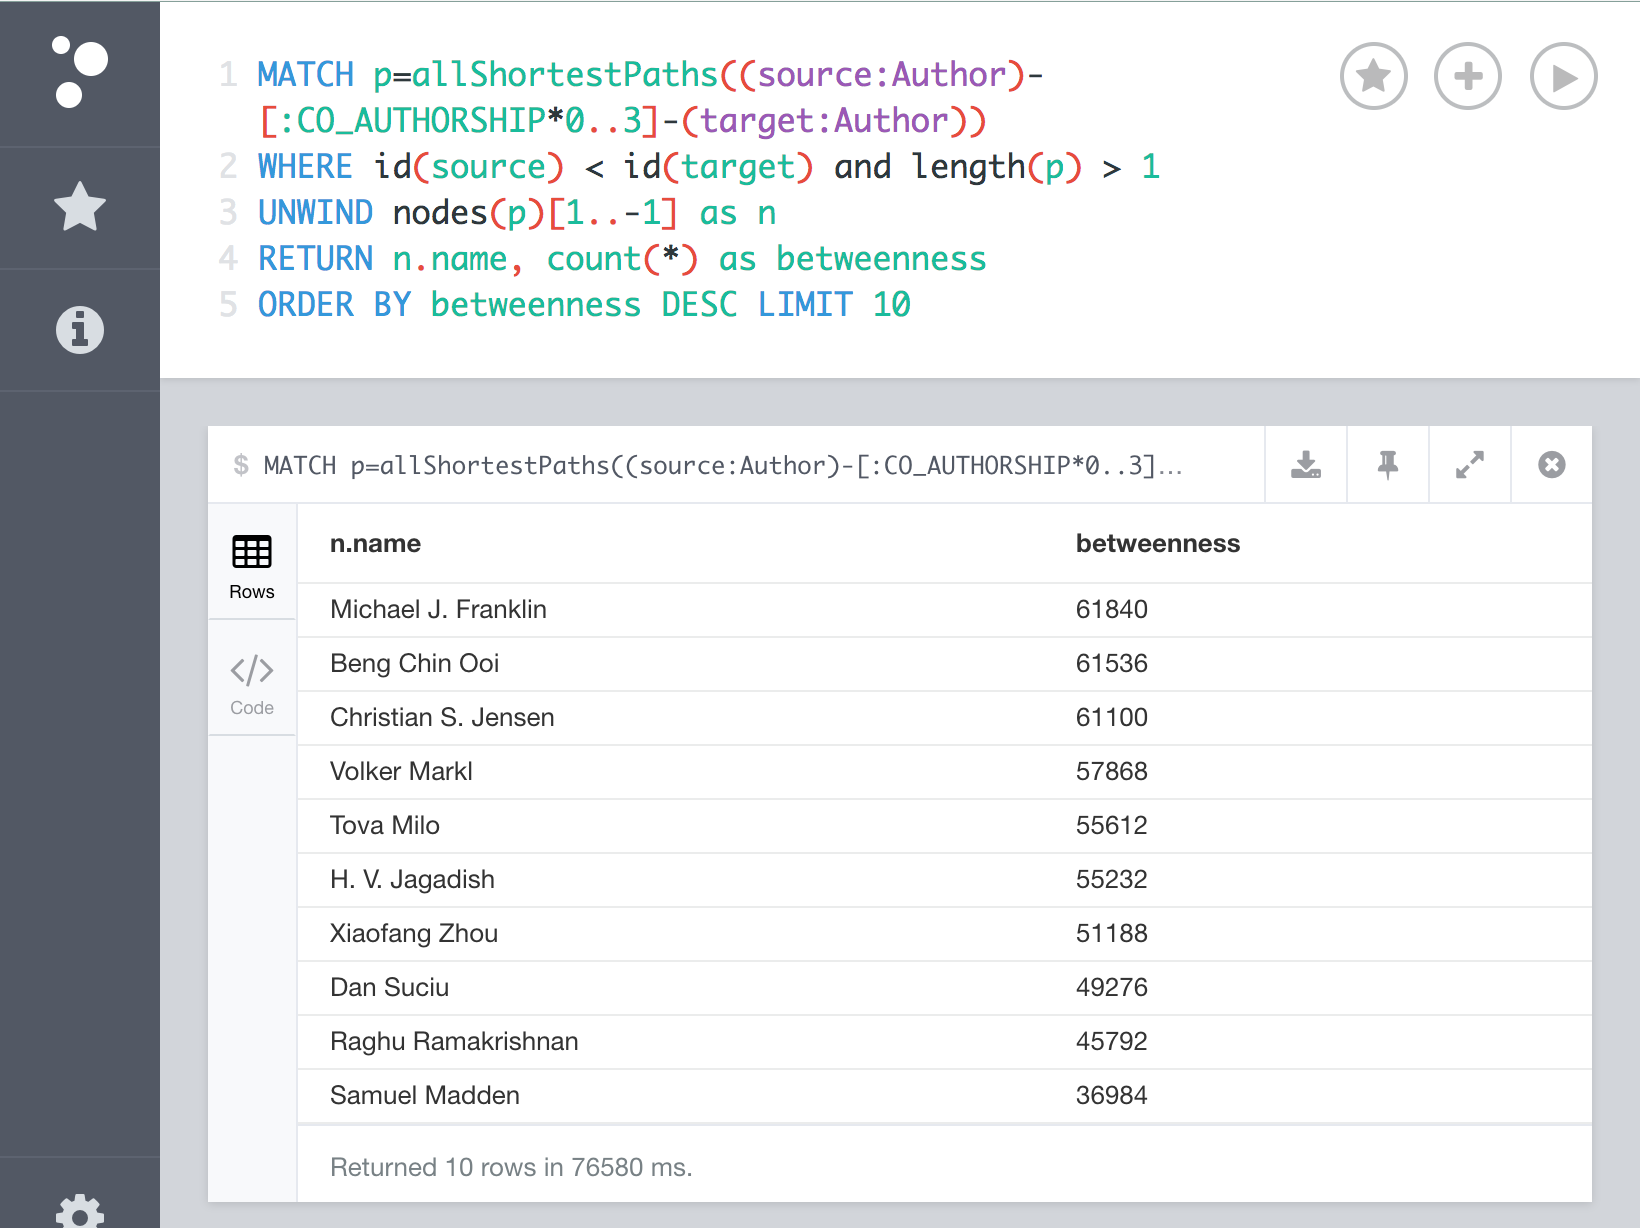
\includegraphics[width=1\textwidth]{../exp_betweenness_centrality.png}
\caption{Result of experiment with the betweenness centrality measure for Authors}
\label{fig:figure36}
\end{figure}

\subsection{Graph as Measure}
This type of measure is given by the aggregate graph itself, since it is a representation of data aggregated by dimensions. For our running example, this measure represents the topological disposition of the relationship between publications and authors when the data is aggregated according to the dimensions year and journal / conference. 

Appendix A shows a screenshot of a subgraph retrieved from the aggregate graph. The subgraph was limited to 400 relationships in order to facilitate the visualisation. From the screenshot we can notice the topology distribution of author nodes that published works on ICDE in 2016 and 2015, specially the authors that published in both editions of the conference.

\section{Results Analysis}
Given the results obtained from the experiments described in the previous section, we are able to confirm the effectiveness of the proposed system in supporting multidimensional analysis on graph database. The presented solution also supports the performance of graph-based analysis, such as centrality measures. In this way we are able to extract three different types of measures from the same origin data aggregated according to user defined dimensions.

In comparison to other works in this area, the proposed system gives full support for heterogeneous graphs without the need to change the original data schema. Focusing the comparison with the framework presented in \cite{Ghrab2013}, our system is able to answer the same types of query without the extra step to change the data model of our original dataset.

\section{Difficulties Found}
Unfortunately, we are unable to provide a more precise comparison between the framework in \cite{Ghrab2013} and the work presented in this chapter due to the lack of experiment description. A similar issue also applies to other works presented in Chapter 3, about the state of the art for Graph Cubes and OLAP analysis on graph databases.

The published papers in this area fail in providing enough description on how the proposed solution was implemented and where the dataset used in the experiments is available. Furthermore, when experiments are presented in the paper, they only compare different version of the same framework. Until now, it hasn't been proposed an experiment that can be performed amongst different frameworks.

The absence of a benchmark for experiments in this area makes the evaluation of the proposed system difficult. In order to compare ourselves to others, we can only rely on qualitative measures, based on the features presented by existing frameworks.

\section{Final Considerations}
In this chapter, we detailed how the system proposed by this work was implemented, specifying what were the technologies used in the process. The dataset used in the experiments was presented as well as the results obtained. Finally, we presented a qualitative comparison with existing solutions and listed the main difficulties found during the system's implementation.

% ----------------------------------------------------------
% ELEMENTOS P�S-TEXTUAIS
% ----------------------------------------------------------
\backmatter
% ----------------------------------------------------------

% ----------------------------------------------------------
% Refer�ncias bibliogr�ficas
% ----------------------------------------------------------
\nocite{*}
\bibliographystyle{alpha}
\bibliography{references}

% ----------------------------------------------------------
% Gloss�rio
% ----------------------------------------------------------
%
% Consulte o manual da classe abntex2 para orienta��es sobre o gloss�rio.
%
%\glossary

% ----------------------------------------------------------
% Ap�ndices
% ----------------------------------------------------------

% ---
% Inicia os ap�ndices
% ---
%\begin{apendicesenv}

%\end{apendicesenv}
% ---


% ----------------------------------------------------------
% Anexos
% ----------------------------------------------------------

% ---
% Inicia os anexos
% ---
%\begin{anexosenv}

%\end{anexosenv}

%---------------------------------------------------------------------
% INDICE REMISSIVO
%---------------------------------------------------------------------
%\phantompart
%\printindex
%---------------------------------------------------------------------

\end{document}
